% Options for packages loaded elsewhere
\PassOptionsToPackage{unicode}{hyperref}
\PassOptionsToPackage{hyphens}{url}
%
\documentclass[
  12pt,
]{article}
\usepackage{amsmath,amssymb}
\usepackage{lmodern}
\usepackage{iftex}
\ifPDFTeX
  \usepackage[T1]{fontenc}
  \usepackage[utf8]{inputenc}
  \usepackage{textcomp} % provide euro and other symbols
\else % if luatex or xetex
  \usepackage{unicode-math}
  \defaultfontfeatures{Scale=MatchLowercase}
  \defaultfontfeatures[\rmfamily]{Ligatures=TeX,Scale=1}
\fi
% Use upquote if available, for straight quotes in verbatim environments
\IfFileExists{upquote.sty}{\usepackage{upquote}}{}
\IfFileExists{microtype.sty}{% use microtype if available
  \usepackage[]{microtype}
  \UseMicrotypeSet[protrusion]{basicmath} % disable protrusion for tt fonts
}{}
\makeatletter
\@ifundefined{KOMAClassName}{% if non-KOMA class
  \IfFileExists{parskip.sty}{%
    \usepackage{parskip}
  }{% else
    \setlength{\parindent}{0pt}
    \setlength{\parskip}{6pt plus 2pt minus 1pt}}
}{% if KOMA class
  \KOMAoptions{parskip=half}}
\makeatother
\usepackage{xcolor}
\usepackage[margin=1in]{geometry}
\usepackage{color}
\usepackage{fancyvrb}
\newcommand{\VerbBar}{|}
\newcommand{\VERB}{\Verb[commandchars=\\\{\}]}
\DefineVerbatimEnvironment{Highlighting}{Verbatim}{commandchars=\\\{\}}
% Add ',fontsize=\small' for more characters per line
\usepackage{framed}
\definecolor{shadecolor}{RGB}{248,248,248}
\newenvironment{Shaded}{\begin{snugshade}}{\end{snugshade}}
\newcommand{\AlertTok}[1]{\textcolor[rgb]{0.94,0.16,0.16}{#1}}
\newcommand{\AnnotationTok}[1]{\textcolor[rgb]{0.56,0.35,0.01}{\textbf{\textit{#1}}}}
\newcommand{\AttributeTok}[1]{\textcolor[rgb]{0.77,0.63,0.00}{#1}}
\newcommand{\BaseNTok}[1]{\textcolor[rgb]{0.00,0.00,0.81}{#1}}
\newcommand{\BuiltInTok}[1]{#1}
\newcommand{\CharTok}[1]{\textcolor[rgb]{0.31,0.60,0.02}{#1}}
\newcommand{\CommentTok}[1]{\textcolor[rgb]{0.56,0.35,0.01}{\textit{#1}}}
\newcommand{\CommentVarTok}[1]{\textcolor[rgb]{0.56,0.35,0.01}{\textbf{\textit{#1}}}}
\newcommand{\ConstantTok}[1]{\textcolor[rgb]{0.00,0.00,0.00}{#1}}
\newcommand{\ControlFlowTok}[1]{\textcolor[rgb]{0.13,0.29,0.53}{\textbf{#1}}}
\newcommand{\DataTypeTok}[1]{\textcolor[rgb]{0.13,0.29,0.53}{#1}}
\newcommand{\DecValTok}[1]{\textcolor[rgb]{0.00,0.00,0.81}{#1}}
\newcommand{\DocumentationTok}[1]{\textcolor[rgb]{0.56,0.35,0.01}{\textbf{\textit{#1}}}}
\newcommand{\ErrorTok}[1]{\textcolor[rgb]{0.64,0.00,0.00}{\textbf{#1}}}
\newcommand{\ExtensionTok}[1]{#1}
\newcommand{\FloatTok}[1]{\textcolor[rgb]{0.00,0.00,0.81}{#1}}
\newcommand{\FunctionTok}[1]{\textcolor[rgb]{0.00,0.00,0.00}{#1}}
\newcommand{\ImportTok}[1]{#1}
\newcommand{\InformationTok}[1]{\textcolor[rgb]{0.56,0.35,0.01}{\textbf{\textit{#1}}}}
\newcommand{\KeywordTok}[1]{\textcolor[rgb]{0.13,0.29,0.53}{\textbf{#1}}}
\newcommand{\NormalTok}[1]{#1}
\newcommand{\OperatorTok}[1]{\textcolor[rgb]{0.81,0.36,0.00}{\textbf{#1}}}
\newcommand{\OtherTok}[1]{\textcolor[rgb]{0.56,0.35,0.01}{#1}}
\newcommand{\PreprocessorTok}[1]{\textcolor[rgb]{0.56,0.35,0.01}{\textit{#1}}}
\newcommand{\RegionMarkerTok}[1]{#1}
\newcommand{\SpecialCharTok}[1]{\textcolor[rgb]{0.00,0.00,0.00}{#1}}
\newcommand{\SpecialStringTok}[1]{\textcolor[rgb]{0.31,0.60,0.02}{#1}}
\newcommand{\StringTok}[1]{\textcolor[rgb]{0.31,0.60,0.02}{#1}}
\newcommand{\VariableTok}[1]{\textcolor[rgb]{0.00,0.00,0.00}{#1}}
\newcommand{\VerbatimStringTok}[1]{\textcolor[rgb]{0.31,0.60,0.02}{#1}}
\newcommand{\WarningTok}[1]{\textcolor[rgb]{0.56,0.35,0.01}{\textbf{\textit{#1}}}}
\usepackage{graphicx}
\makeatletter
\def\maxwidth{\ifdim\Gin@nat@width>\linewidth\linewidth\else\Gin@nat@width\fi}
\def\maxheight{\ifdim\Gin@nat@height>\textheight\textheight\else\Gin@nat@height\fi}
\makeatother
% Scale images if necessary, so that they will not overflow the page
% margins by default, and it is still possible to overwrite the defaults
% using explicit options in \includegraphics[width, height, ...]{}
\setkeys{Gin}{width=\maxwidth,height=\maxheight,keepaspectratio}
% Set default figure placement to htbp
\makeatletter
\def\fps@figure{htbp}
\makeatother
\setlength{\emergencystretch}{3em} % prevent overfull lines
\providecommand{\tightlist}{%
  \setlength{\itemsep}{0pt}\setlength{\parskip}{0pt}}
\setcounter{secnumdepth}{5}
\newlength{\cslhangindent}
\setlength{\cslhangindent}{1.5em}
\newlength{\csllabelwidth}
\setlength{\csllabelwidth}{3em}
\newlength{\cslentryspacingunit} % times entry-spacing
\setlength{\cslentryspacingunit}{\parskip}
\newenvironment{CSLReferences}[2] % #1 hanging-ident, #2 entry spacing
 {% don't indent paragraphs
  \setlength{\parindent}{0pt}
  % turn on hanging indent if param 1 is 1
  \ifodd #1
  \let\oldpar\par
  \def\par{\hangindent=\cslhangindent\oldpar}
  \fi
  % set entry spacing
  \setlength{\parskip}{#2\cslentryspacingunit}
 }%
 {}
\usepackage{calc}
\newcommand{\CSLBlock}[1]{#1\hfill\break}
\newcommand{\CSLLeftMargin}[1]{\parbox[t]{\csllabelwidth}{#1}}
\newcommand{\CSLRightInline}[1]{\parbox[t]{\linewidth - \csllabelwidth}{#1}\break}
\newcommand{\CSLIndent}[1]{\hspace{\cslhangindent}#1}
\ifLuaTeX
\usepackage[bidi=basic]{babel}
\else
\usepackage[bidi=default]{babel}
\fi
\babelprovide[main,import]{spanish}
% get rid of language-specific shorthands (see #6817):
\let\LanguageShortHands\languageshorthands
\def\languageshorthands#1{}
\usepackage{dcolumn}
\usepackage{rotating}
\usepackage{xcolor}
\usepackage[bottom]{footmisc}
\usepackage{setspace}
\usepackage{multirow}
\usepackage{footnote}
\usepackage{caption}
\usepackage{subcaption}
\usepackage[font=small,labelfont=it,margin=\parindent,tableposition=top]{caption}
\usepackage{booktabs}
\usepackage{longtable}
\usepackage{array}
\usepackage{multirow}
\usepackage{wrapfig}
\usepackage{float}
\usepackage{colortbl}
\usepackage{pdflscape}
\usepackage{tabu}
\usepackage{threeparttable}
\usepackage{threeparttablex}
\usepackage[normalem]{ulem}
\usepackage{makecell}
\usepackage{xcolor}
\ifLuaTeX
  \usepackage{selnolig}  % disable illegal ligatures
\fi
\IfFileExists{bookmark.sty}{\usepackage{bookmark}}{\usepackage{hyperref}}
\IfFileExists{xurl.sty}{\usepackage{xurl}}{} % add URL line breaks if available
\urlstyle{same} % disable monospaced font for URLs
\hypersetup{
  pdflang={es-CO},
  hidelinks,
  pdfcreator={LaTeX via pandoc}}

\author{}
\date{\vspace{-2.5em}}

\begin{document}

Título cool

\newpage

\newpage
\begin{spacing}{0.9} 
\tableofcontents
\end{spacing}

\newpage

\begin{spacing}{0.9} 
\listoftables
\end{spacing}

\newpage
\listoffigures
\newpage
\normalsize

\hypertarget{introducciuxf3n}{%
\section{Introducción}\label{introducciuxf3n}}

\pagebreak

\hypertarget{literatura-sobre-emotividad-y-polarizaciuxf3n}{%
\section{Literatura sobre emotividad y
polarización}\label{literatura-sobre-emotividad-y-polarizaciuxf3n}}

\pagebreak

\hypertarget{fuentes-de-informaciuxf3n-y-preprocesamiento}{%
\section{Fuentes de información y
preprocesamiento}\label{fuentes-de-informaciuxf3n-y-preprocesamiento}}

Esta sección describe las principales características del dataset
utilizado y los procedimientos realizados durante la etapa de
preprocesamiento. Los datos provienen de tres fuentes de información: 1)
textos parlamentarios emitidos desde 1965 a 2022; 2) biografías
parlamentarias y 3) votaciones dentro de la cámara de diputados desde
2002 a 2022.

\hypertarget{textos-parlamentarios-biblioteca-del-congreso-nacional}{%
\subsection{Textos parlamentarios biblioteca del congreso
nacional}\label{textos-parlamentarios-biblioteca-del-congreso-nacional}}

Los textos parlamentarios corresponden a todas las transcripciones de
intervenciones parlamentarias realizadas en ambas cámaras desde el año
1965 hasta 2022. Debido a que actualmente no existe un set de datos
ordenado de los discursos parlamentarios, la información fue obtenida
del sitio web de la Biblioteca del Congreso Nacional por medio de
técnicas de
\emph{webscraping}\footnote{En concreto, se desarrolló un código en R y por medio de una tecnología llamada Selenium se simuló un usuario que navegó a través de todos los discursos parlamentarios durante varias horas.}.
De esta manera, fueron obtenidas las transcripciones íntegras, junto a
algunos metadatos disponibles, como el título de la intervención, fecha
y autores de la misma.

La recolección de información tuvo como resultado un total de 579.663
intervenciones parlamentarias (tabla \ref{tab:tabla_pre_post_filtro}),
tanto individuales como grupales. Luego de una edición y selección de
intervenciones relevantes, el dataset final quedó conformado por 209.830
textos. Existen dos motivos que explican la reducción en la cantidad de
registros. En primer lugar, se seleccionaron aquellas intervenciones en
las que participa un solo parlamentario, de modo de asociar claramente
un discurso a una
persona\footnote{Es común que una misma intervención esté firmada por dos o más parlamentarios}.
El segundo motivo guarda relación con la remoción de ciertas categorías
de intervenciones parlamentarias que no son de interés para el presente
estudio. Existen 52 categorías de participaciones parlamentarias, muchas
de las cuales corresponden a asuntos administrativos o tienen un
lenguaje con un fuerte sesgo técnico-jurídico. Dichas intervenciones
fueron removidas, puesto que no están asociados al objetivo de este
trabajo\footnote{Para más detalle sobre las categorías de participaciones parlamentarias ver Anexo}

\begin{table}[H]

\caption{\label{tab:tabla_pre_post_filtro}Total de intervenciones parlamentarias}
\centering
\begin{tabular}[t]{ll}
\toprule
filtro & cantidad de filas\\
\midrule
datos brutos & 579.663\\
datos filtrados & 209.830\\
\bottomrule
\end{tabular}
\end{table}

Tal como muestra la figura \ref{n_year}, existe una ventana de 17 años
en la que no se cuenta con información debido al cierre del Congreso
Nacional durante la
dictadura\footnote{No se muestran los datos de 2022 en el gráfico debido al bajo número de intervenciones existen en el momento de la recolección de información. Esta fue realizada durante marzo de 2022, de modo que a dicha fecha solo se registra una pequeña fracción de las intervenciones que usualmente se llevan a cabo durante un año legislativo}.

\begin{figure}[H]
\centering
\large
\caption{Número de intervenciones parlamentarias por año}
\label{n_year}
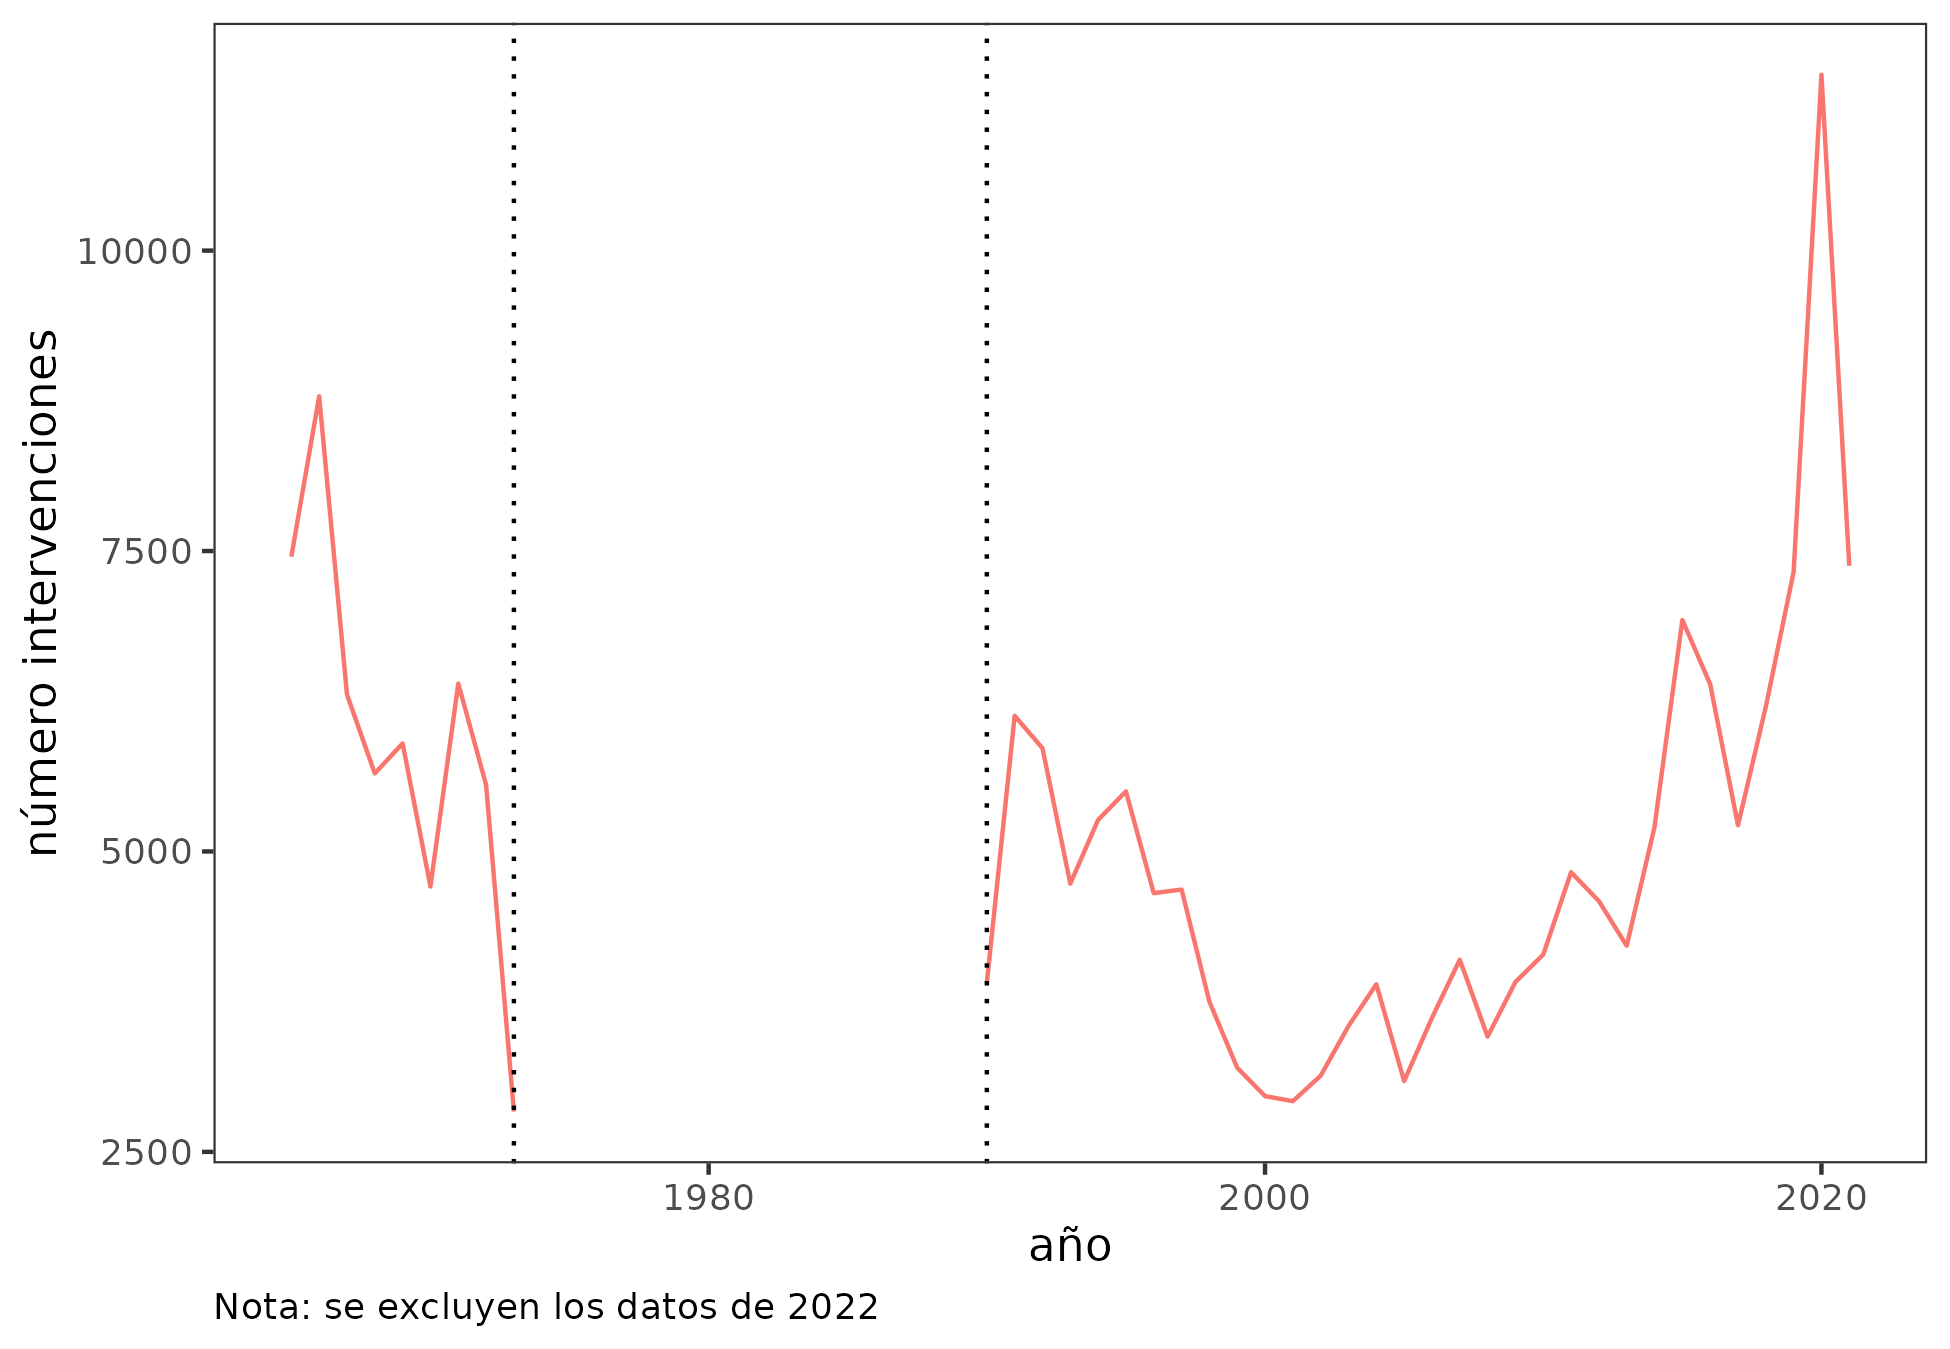
\includegraphics[width = 0.5 \textwidth]{cuadros_tesis/plot_n_year.png}
\normalsize
\end{figure}

Con el objeto de convertir los discursos parlamentarios en información
estadísticamente relevante, fue necesario llevar a cabo un pre
procesamiento de los datos. En primer lugar, se convirtieron todos los
textos a minúscula, lo cual facilita una serie de tareas posteriores y
reduce el número de palabras únicas. En segundo lugar, se removieron
algunos extractos de los textos poco informativos, como los vocativos u
otros encabezados
similares\footnote{Una gran cantidad de discursos comienza con el vocativo  \textit{señor presidente} o \textit{señora presidenta}. Otro caso muy común se da cuando el presidente o presidenta de la Cámara cede la palabra a un parlamentario, en cuyo caso suele utilizarse la fórmula \textit{el/la diputado/a [nombre] tiene la palabra}}.

En tercer lugar, se dividieron los discursos en
párrafos\footnote{El separador utilizado fue el interlineado}, los
cuales constituyen la unidad de análisis que da lugar a los resultados
de este trabajo. Una vez separados en párrafos, los textos fueron
separados (\emph{tokenizados}) en palabras.

En cuarto lugar, se removieron los signos de puntuación y las palabras
que en la terminología de NLP se denominan \emph{stopwords}. Estas
palabras se caracterizan por ser muy comunes, pues al corresponder a una
parte estructural de los idiomas, se utilizan en prácticamente todos los
contextos, por ende, para muchas tareas de clasificación de textos no
aportan información relevante. Por lo general, las librerías utilizadas
para NLP contienen listados de \emph{stopwords}. Estos listados,
típicamente, incluyen conjunciones, preposiciones, algunos adverbios y
otras partículas.

Finalmente, se seleccionan los sustantivos, adjetivos y verbos mediante
un modelo de
\emph{spacy}\footnote{Spacy es una librería de Python ampliamente utilizada para facilitar tareas relacionadas con el procesamiento de lenguaje natural. Spacy contiene modelos para hacer POS, *name entity recognition*, mapeo de palabras a vectores, entre otras herramientas}
entrenado para hacer POS (\emph{Part of speech}). Mediante esta
operación se busca retener aquellas palabras que aportan más significado
al contenido de los discursos parlamentarios, lo cual, además, disminuye
el tiempo de computación, ya que se elimina una parte importante de las
palabras del corpus.

El cuadro \ref{tab:ejemplo_preprocesamiento} muestra un ejemplo de la
situación inicial y final de un extracto de una de las intervenciones
parlamentarias. Es posible observar lo siguiente: 1) el texto final está
en minúscula, 2) no existen signos de puntuación, 3) varias palabras han
sido removidas y 4) el párrafo original está contenido en una lista de
palabras.

\begin{table}[H]

\caption{\label{tab:ejemplo_preprocesamiento}Ejemplo de preprocesamiento}
\centering
\begin{tabular}[t]{>{\raggedright\arraybackslash}p{15em}>{\raggedright\arraybackslash}p{15em}}
\toprule
original & final\\
\midrule
\em{\textbf{Lo destaco, porque queremos trabajar en los proyectos de los parlamentarios. Hemos visto lo que se busca con este proyecto, el ministro de Hacienda ya había anticipado que queremos aliviar  a las familias en materia crediticia y compartimos el espíritu de lo que se quiere. Y eso es justamente lo que explica  que queramos trabajar sobre los diversos proyectos de ley que ustedes han empujado y han sacado adelante.}} & \em{\textbf{{}['destaco', 'queremos', 'trabajar', 'proyectos', 'parlamentarios', 'visto', 'busca', 'proyecto', 'ministro',  'anticipado', 'queremos', 'aliviar', 'familias', 'materia', 'crediticia', 'compartimos', 'espíritu',  'quiere', 'explica', 'queramos', 'trabajar', 'proyectos', 'ley', 'empujado', 'sacado']}}\\
\bottomrule
\end{tabular}
\end{table}

Para tener una idea general de las características del dataset, el
cuadro \ref{tab:descripcion_dataset} muestra algunos estadísticos de
resumen. Las 209.830 intervenciones, al ser separadas en unidades más
pequeñas, dan lugar a un total de 2.649.588 de párrafos, cuya media de
palabras es de .

\begin{table}[H]

\caption{\label{tab:descripcion_dataset}Estadísticos de resumen}
\centering
\begin{tabular}[t]{lllll}
\toprule
total intervenciones & total párrafos & total palabras & intervención/párrafos & intervención/palabras\\
\midrule
209.830 & 2.649.588 & 49.065.194 & 12,63 & 233,83\\
\bottomrule
\end{tabular}
\end{table}

Respecto a los párrafos (unidad de análisis), el cuadro
\ref{tab:descripcion_parrafos} y la figura
\ref{plot_descripcion_parrafos} muestran que el número promedio de
palabras es aproximadamente 19 y que, en general, los textos no son
demasiado extensos, ya que el 50\% tiene 15 palabras o menos y el 90\%
tiene 39 palabras o menos. El hecho de utilizar una unidad de análisis
más desagregada que la intervención (párrafo), hace más sencilla la
identificación en el texto de características distintivas, las cuales
cuales tienden a oscurecerse al trabajar con los textos completos, cuya
extensión es significativamente mayor, como se muestra en la tabla
\ref{tab:descripcion_dataset}.

\begin{table}[H]

\caption{\label{tab:descripcion_parrafos}Estadísticos de resumen de los párrafos}
\centering
\begin{tabular}[t]{rrrrr}
\toprule
media & mediana & mínimo & máximo & p90\\
\midrule
18.52 & 15 & 1 & 790 & 39\\
\bottomrule
\end{tabular}
\end{table}

\begin{figure}[H]
\centering
\large
\caption{Histograma del número de palabras por párrafo}
\label{plot_descripcion_parrafos}
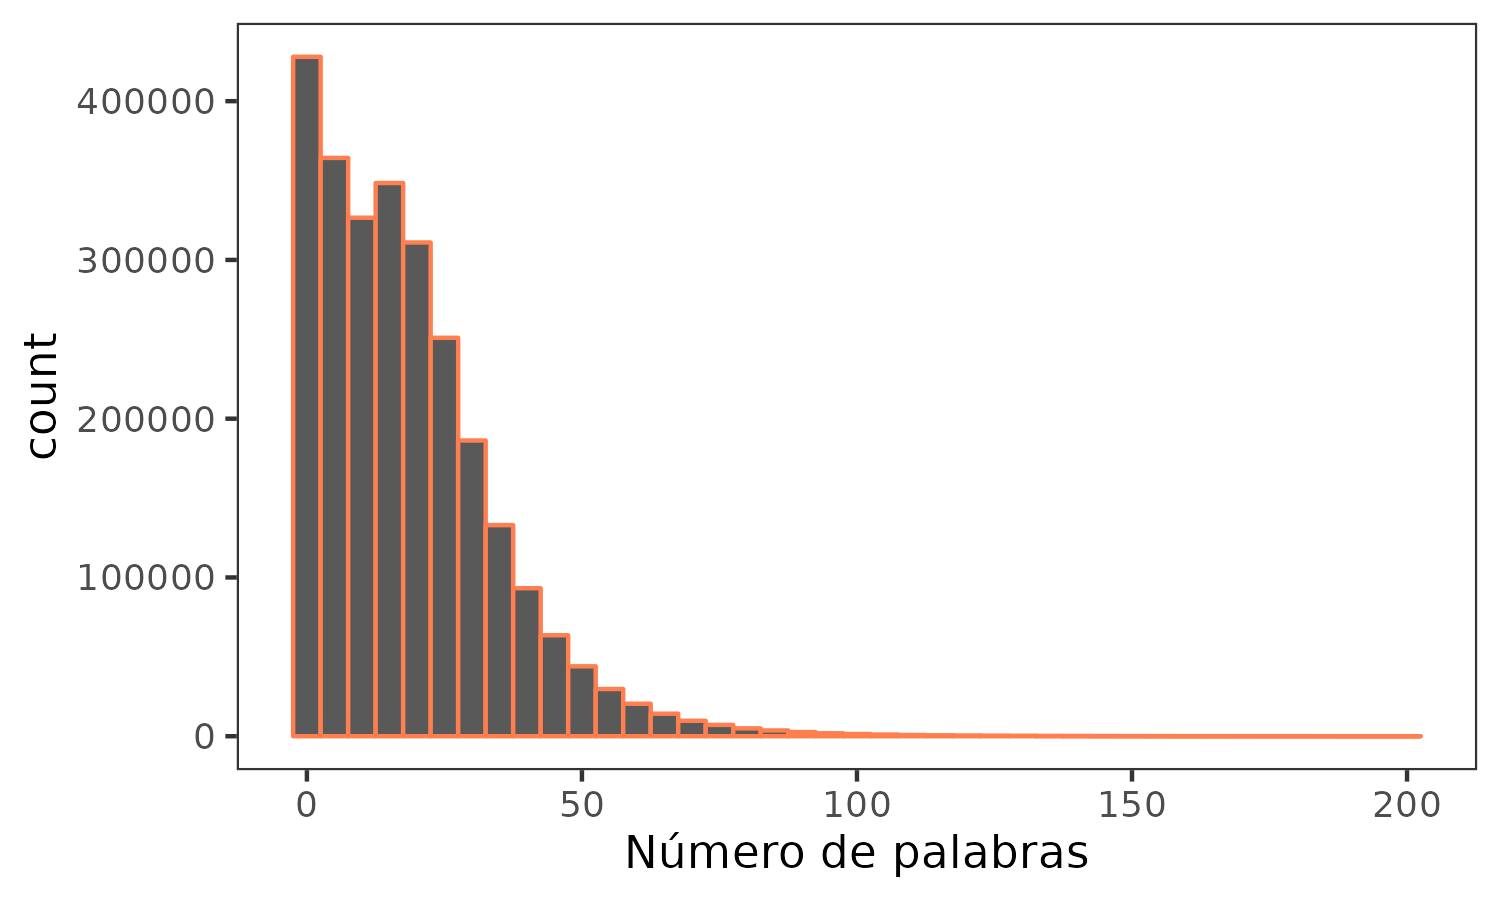
\includegraphics[width = 0.5 \textwidth]{cuadros_tesis/plot_hist_descripcion_parrafos.png}
\normalsize
\end{figure}

\hypertarget{biografuxedas-parlamentarias-biblioteca-del-congreso-nacional}{%
\subsection{Biografías parlamentarias biblioteca del congreso
nacional}\label{biografuxedas-parlamentarias-biblioteca-del-congreso-nacional}}

Para obtener la historia de militancia política de los parlamentarios,
se utilizaron las biografías publicadas en el sitio de la Biblioteca del
Congreso Nacional. Al igual que en el caso de las intervenciones, la
información fue extraída mediante técnicas de \emph{webscraping}.

Una vez finalizada la extracción de datos, fue posible reconstruir la
historia de afiliación política de cada uno de los parlamentarios. A
partir de esta información, cada intervención parlamentaria puede ser
asociada a una militancia específica. Es relevante constatar que dado
que algunos parlamentarios presentan cambios en su militancia, es
posible que dos textos enunciados por la misma persona en momentos
distintos, estén asociados a partidos políticos diferentes.

\hypertarget{votaciones-de-diputados}{%
\subsection{Votaciones de diputados}\label{votaciones-de-diputados}}

La última fuente de información corresponde a las votaciones en sala de
los parlamentarios. Para obtener estos datos se utilizó una API
(\emph{Application Programming Interface}) dispuesta por la Cámara de
Diputados, mediante la cual fue posible extraer todas las votaciones
emitidas en la cámara baja desde 2002 en adelante. Es importante
mencionar dos limitaciones respecto a esta fuente de información:

\begin{enumerate}
\def\labelenumi{\arabic{enumi}.}
\item
  Solo fue posible obtener las votaciones para diputados en la ventana
  de tiempo que va de 2002 a 2022, pues la base de datos dispuesta por
  la Cámara de Diputados solo contiene datos a partir de dicho año.
\item
  No se cuenta con datos de votación para senadores. El motivo es que el
  \emph{web service} del Senado no incluye un método para descargar
  dichos datos.
\end{enumerate}

Estas brechas de información son parte de las limitaciones del estudio,
ya que no es posible descartar que la ausencia de datos más antiguos
para diputados y la inexistencia de datos para senadores, esté
introduciendo algún sesgo en los resultados.

La descarga desde la API tuvo como resultado un total de 20.271
votaciones, distribuidas a lo largo de aproximadamente 20 años. Estos
datos permiten conocer cuál es la situación de todos los diputados en
cada una de las votaciones, pudiendo darse 4 posibilidades:
\emph{aprobación}, \emph{rechazo}, \emph{abstención} o
\emph{dispensado}. La figura \ref{plot_n_votaciones} muestra una
tendencia creciente en el número de votaciones por año a lo largo del
tiempo. A partir de estos datos se construyó una medida de
posicionamiento político que se describe en el apartado
\ref{apartado_nominate}.

\begin{figure}[H]
\centering
\large
\caption{Cantidad de votaciones por año en la Cámara de Diputados}
\label{plot_n_votaciones}
\includegraphics[width = 0.5 \textwidth]{cuadros_tesis/plot_n_votaciones.png}
\normalsize
\end{figure}

\newpage

\hypertarget{metodologuxeda}{%
\section{Metodología}\label{metodologuxeda}}

Esta sección describe los aspectos metodológicos más importantes que se
encuentran a la base de los datos presentados en el apartado de
resultados. Se entregan las principales características del diccionario
utilizado, la metodología de \emph{word embeddings} y cómo es que esta
es utilizada para ubicar cada texto en la polaridad cognitiva-afectiva.

\hypertarget{word-embeddings}{%
\subsection{\texorpdfstring{Word embeddings
\label{word_emb}}{Word embeddings }}\label{word-embeddings}}

El procesamiento y análisis de datos de texto comúnmente requiere llevar
a cabo alguna operación para convertir el lenguaje humano en una
representación numérica que sea legible para un algoritmo. Cualquier
procedimiento que permita convertir palabras en vectores numéricos se
denomina \emph{word embeddings} (Skansi 2018).

Dentro de las estrategias para construir vectores de palabras, una de
las más utilizadas es el modelo \emph{Word2vec}, cuya idea fundamental
es que el significado de una palabra depende del contexto en el que esta
se encuentre. Siguiendo dicha noción, para aprender vectores de
palabras, se entrena una red neuronal utilizando grandes volúmenes de
texto, lo cual se puede llevar a cabo mediante dos estrategias
alternativas: CBOW (\emph{Continues Bag of Words}) o \emph{skip-gram}
(Charu C. 2018). En el modelo CBOW se entrena una red neuronal para que
prediga una palabra a partir de su contexto. Al contrario, en el enfoque
\emph{skip-gram} se utiliza una palabra para predecir el contexto.

Si se define que el contexto corresponde a dos palabras, en CBOW
utilizaremos las dos palabras anteriores y las dos posteriores para
predecir una palabra central. A la inversa, bajo la estrategia
\emph{skip-gram} se utiliza como entrada la palabra central, para
predecir las dos anteriores y dos posteriores.

En términos de arquitectura, los modelos están conformados por una capa
de entrada, una capa oculta y una capa de salida. La capa oculta
determina la cantidad de dimensiones que tendrán los vectores de
palabras. De este modo, si la capa oculta contiene 100 neuronas, el
número de dimensiones para representar cada palabra será 100. Cabe
señalar que tanto la capa de entrada como la de salida tienen el mismo
número de dimensiones, correspondiente a la cantidad de palabras
distintas en el corpus utilizado para llevar a cabo el entrenamiento.

Los modelos descritos no se diferencian en lo fundamental de los
autocodificadores (\emph{autoencoders}): se busca llevar a cabo un
aprendizaje no supervisado (Skansi 2018), lo cual es posible gracias a
la disponibilidad de grandes volúmenes de texto. Ahora bien, debido a
que el proceso de entrenamiento por lo general es costoso, es común la
utilización de modelos desarrollados por personas u organizaciones que
cuentan con \emph{hardware} adecuado para este tipo de tareas.

En el marco de este trabajo se utilizaron los vectores entrenados por
(Perez y Cañete 2019) del Departamento de Ciencias de la Computación de
la Universidad de Chile. Los autores utilizan el algoritmo
\emph{FastText} (Bojanowski et~al. 2016) sobre un corpus en español
llamado \emph{Spanish Unannotated Corpora}
(SUC)\footnote{Corpus construido a partir de una gran cantidad de fuentes. El dataset está conformado por 300 millones de líneas. Para mayores detalles sobre el dataset, ver https://github.com/josecannete/spanish-corpora}.
\emph{FastText} recoge la idea de que es posible capturar el significado
de las palabras a partir de sus contextos, sin embargo, se diferencia de
\emph{Word2Vec} en el hecho de que el texto no es dividido en palabras,
sino en conjuntos de caracteres más pequeños. El significado se
construye en este caso a partir de cadenas de caracteres que componen
las palabras. Ello hace posible, entre otras cosas, obtener vectores
para cualquier palabra, independiente de que estas hayan estado o no
presentes en el corpus de entrenamiento.

Pérez y Cañete (2019) ponen a disposición varios modelos, cuya
diferencia principal dice relación con el número de dimensiones que
tienen los vectores. El más pequeño está conformado por vectores de 10
dimensiones, mientras que el más grande, por vectores de 300
dimensiones. Con el objeto de facilitar el procesamiento de datos, en
esta investigación se utiliza un modelo de 100 dimensiones. Cabe señalar
que si bien los vectores de 300 dimensiones debiesen reflejar de mejor
manera el significado de las palabras, el modelo de 100 dimensiones
ofrece resultados satisfactorios a un costo de procesamiento
significativamente menor.

Los vectores de palabras construidos mediante \emph{FastText} y
\emph{Word2Vec} han demostrado ser capaces de capturar el significado de
las palabras. Así, palabras que aparecen en contextos similares, estarán
cerca en el espacio proyectado, lo cual implica que es posible llevar a
cabo operaciones algebraicas y agrupar palabras según la dirección en la
que apunten los vectores. Por ejemplo, si buscamos los vectores más
cercanos a \emph{rojo} (mediante similitud coseno u otra medida de
distancia), utilizando el modelo de 100 dimensiones, se observa que el
resultado corresponde a otros colores.

\begin{Shaded}
\begin{Highlighting}[]
\NormalTok{colores }\OperatorTok{=}\NormalTok{  wordvectors.most\_similar(positive}\OperatorTok{=}\NormalTok{[}\StringTok{\textquotesingle{}rojo\textquotesingle{}}\NormalTok{],  topn }\OperatorTok{=} \DecValTok{5}\NormalTok{)}
\end{Highlighting}
\end{Shaded}

\begin{table}[H]

\caption{\label{tab:tabla_colores}Palabras más cercanas a rojo}
\centering
\begin{tabular}[t]{lr}
\toprule
palabra & similitud\\
\midrule
amarillo & 0.906\\
azul & 0.903\\
blanco & 0.866\\
negro & 0.853\\
anaranjado & 0.843\\
\bottomrule
\end{tabular}
\end{table}

La idea de que las palabras cercanas tienen un correlato en el espacio
se puede expresar de manera gráfica mediante un ejercicio de reducción
de dimensionalidad. La figura \ref{plot_pca_ejemplo} corresponde a las
dos primeras componentes de un Análisis de Componentes Principales
(PCA). Se puede observar que al proyectar los vectores en este nuevo
espacio de dos dimensiones, las posiciones de las palabras generan
agrupaciones conceptuales. De hecho, podemos observar tres grupos
claramente definidos: animales, colores y comidas.

\begin{figure}[H]
\centering
\large
\caption{Agrupación de palabras en un espacio bidimensional}
\label{plot_pca_ejemplo}
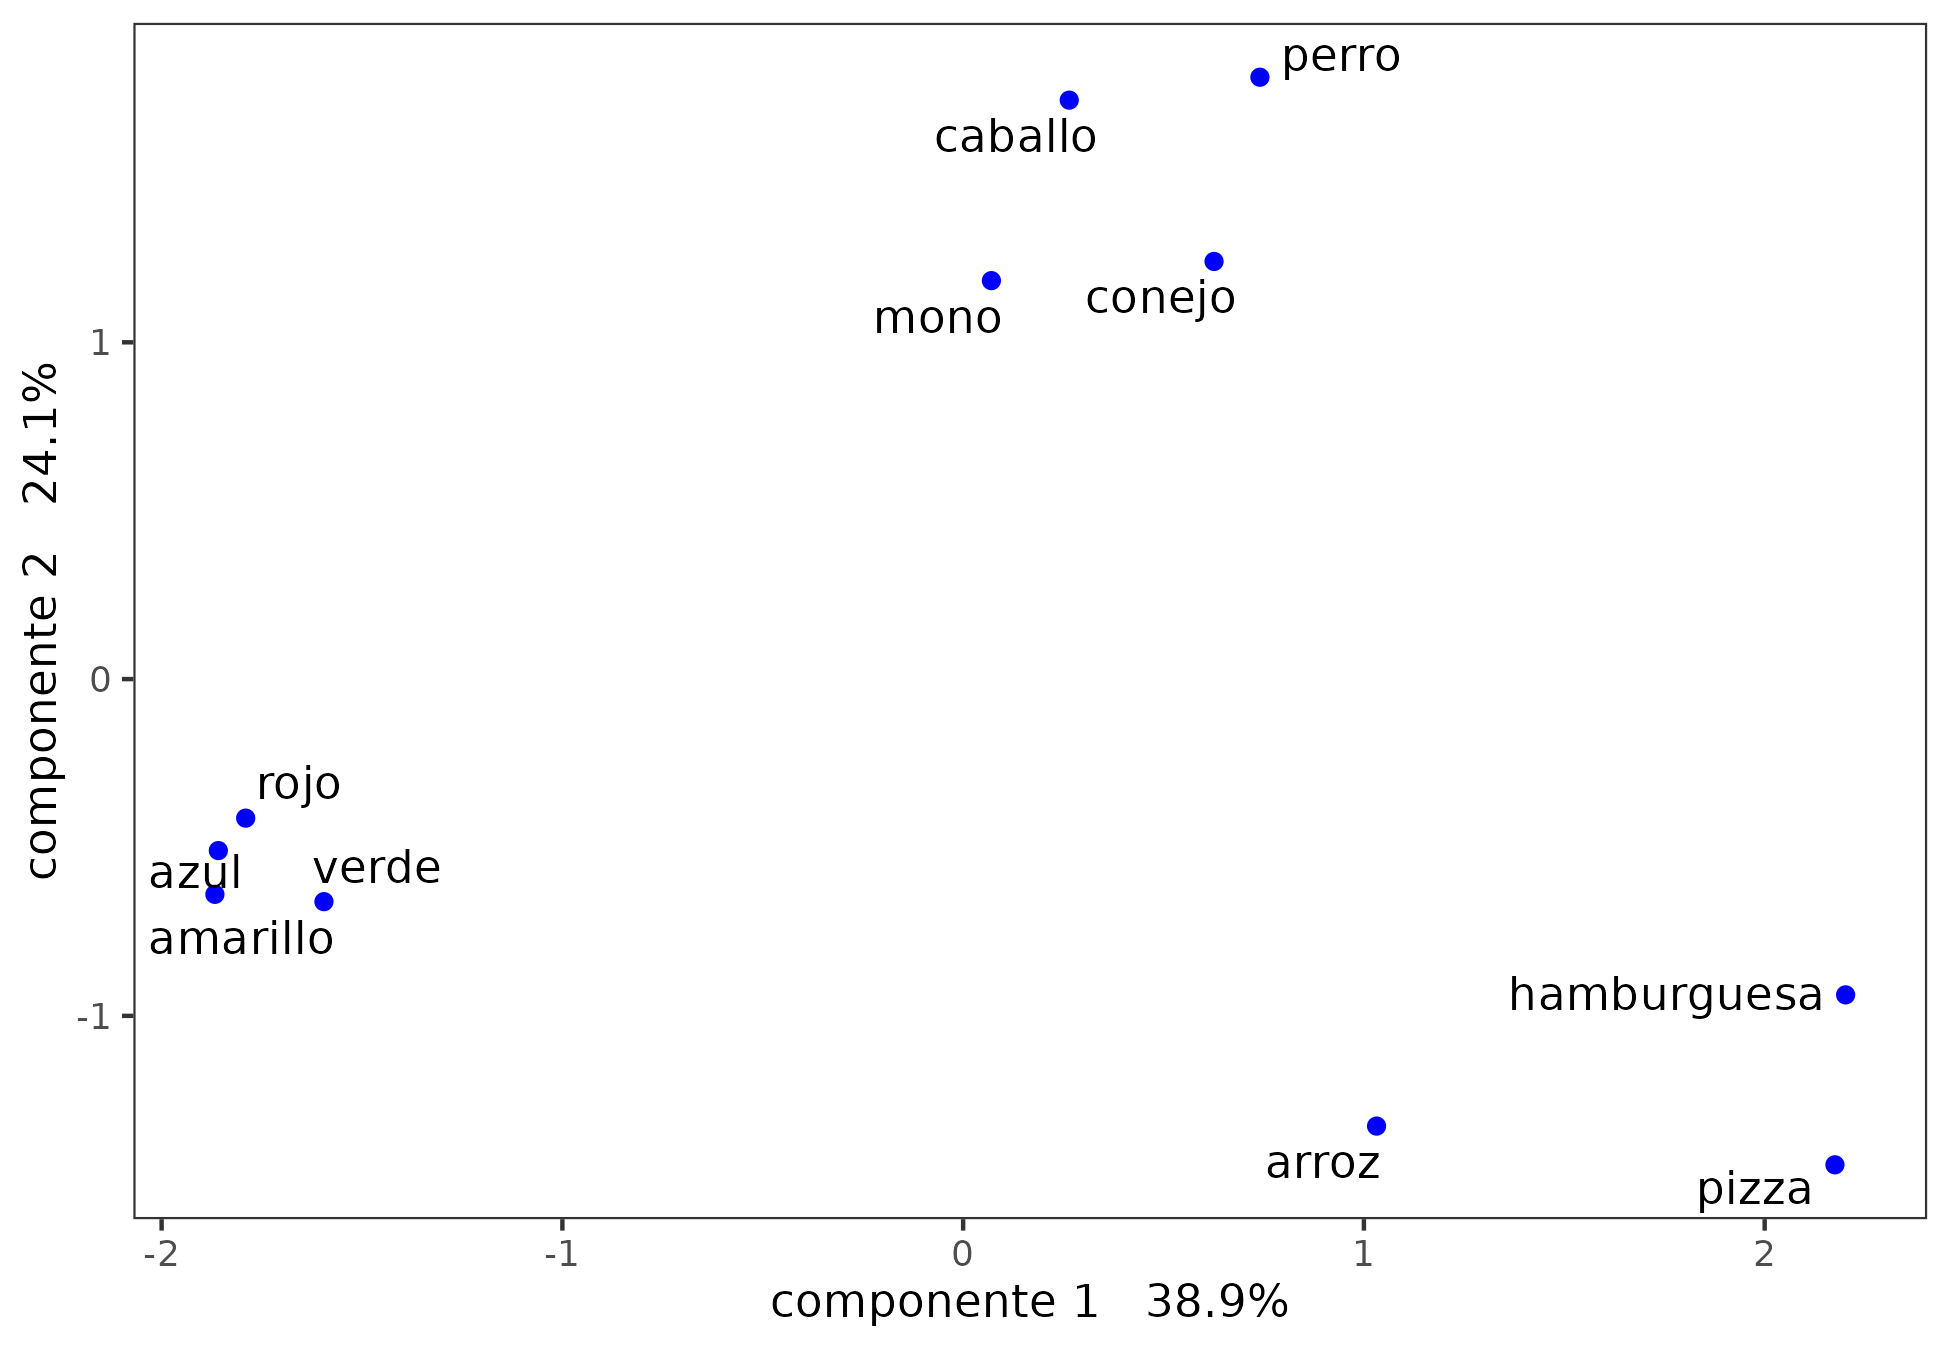
\includegraphics[width = 0.5 \textwidth]{cuadros_tesis/plot_pca.png}
\normalsize
\end{figure}

Los vectores también permiten construir analogías del tipo \(a\) es a
\(b\) como \(x\) es a \(y\) y establecer operaciones como la siguiente:

\begin{align}
\label{analogia_formula}
reina \approx rey - hombre + mujer
\end{align}

La ecuación \ref{analogia_formula} es una manera de representar
algebráicamente la relación
\textit{hombre es a rey, como mujer es a reina}. Mediante alguna medida
de distancia (usualmente, similitud coseno) se busca el vector más
cercano a \(rey\) y a \(mujer\) y que, al mismo tiempo, se aleje del
vector \(hombre\). La tabla \ref{tab:ejemplo_analogia} muestra que el
vector más parecido, efectivamente, corresponde a \emph{reina}, seguido
por \emph{princesa} y otras palabras que podrían ajustarse a la
analogía. En ese sentido, los vectores permiten construir relaciones
semánticas complejas y, por ende, son útiles para representar el
lenguaje humano.

\begin{table}[H]

\caption{\label{tab:ejemplo_analogia}Ejemplo de analogía con Word Embeddings. 5 palabras más cercanas a la analogía}
\centering
\begin{threeparttable}
\begin{tabular}[t]{l>{\raggedright\arraybackslash}p{20em}}
\toprule
palabra & similitud coseno\\
\midrule
reina & 0.763\\
princesa & 0.665\\
consorte & 0.665\\
sibila & 0.653\\
isabel & 0.650\\
\bottomrule
\end{tabular}
\begin{tablenotes}[para]
\small
\item \textit{Nota:} 
\item Se calcula similitud coseno entre el vector resultante de la ecuación 1 y todos los demás vectores. La tabla presenta las 5 palabras más cercanas a dicho vector
\end{tablenotes}
\end{threeparttable}
\end{table}

Es importante mencionar que una estrategia alternativa a la de
\emph{word embeddings} es utilizar un listado de palabras previamente
clasificadas e identificar cada aparición de estas en los textos. Una
vez hecho lo anterior, es posible construir una medida sintética para
cada documento mediante alguna operación de agregación, como suma
simple, suma ponderada u otro procedimiento similar. Existen al menos
dos grandes ventajas de utilizar el enfoque de \emph{word embeddings} en
lugar de estrategias que busquen simplemente la presencia o ausencia de
palabras en un texto.

\begin{enumerate}
\def\labelenumi{\arabic{enumi}.}
\item
  No se requiere un \emph{match} exacto de palabras, ya que es posible
  trabajar con la noción de distancia en un espacio vectorial. A modo de
  ejemplo, si un diccionario contiene la palabra \emph{rabia} y no la
  palabra \emph{ira} y se intenta clasificar el texto \emph{los
  políticos a veces sienten ira}, el enfoque de \emph{word embeddings}
  será capaz de detectar que la palabra \emph{ira} apunta hacia una
  dirección cercana a \emph{rabia}, asignando un puntaje conforme a
  alguna medida de distancia. Al contrario, una estrategia que considere
  únicamente la presencia de una palabra, no podrá asignar puntaje.
\item
  No se requiere establecer \emph{a priori} el puntaje de cada palabra
  del diccionario. Inevitablemente, al utilizar diccionarios surge la
  pregunta sobre la intensidad de una palabra respecto a algún concepto.
  Por ejemplo, ¿las palabras amistad y amor deberían tener el mismo
  puntaje de afectividad? Existen diccionarios, como AFINN (Nielsen
  2011), SentiWordNet o VADER (Hutto y Gilbert 2014), que establecen
  puntajes en la polaridad negativo-positivo, utilizando una metodología
  basada en jueces. Esto hace surgir preguntas respecto al modo en que
  el puntaje fue asignado: ¿Cuántos jueces deben votar? ¿Qué palabras
  deben seleccionarse? ¿Qué escala se utilizará?, etc. Otra estrategia
  posible es que todas las palabras tengan puntaje igual a 1, de modo de
  evaluar simplemente la presencia o ausencia de las mismas en un texto,
  como se hace en el diccionario Bing (Hu y Liu 2004), sin embargo,
  asignar el mismo puntaje no resuelve el problema, pues ello también es
  una ponderación (todas las palabras tienen la misma ponderación).
\end{enumerate}

El enfoque de \emph{word embeddings} no requiere lidiar con este tipo de
decisiones, ya que el vector que representa una palabra contiene su
significado. En ese sentido, si el entrenamiento funcionó y los vectores
efectivamente dan cuenta del significado de las palabras, entonces, no
es necesario tomar decisiones respecto a la asignación de ponderaciones.
En términos empíricos, Gennaro y Ash (2021) entregan evidencia de que
una estrategia basada en \emph{word embeddings} genera mejores
resultados que una estrategia basada un \emph{match} exacto de palabras,
para el análisis de textos parlamentarios en EEUU.

\hypertarget{diccionario-liwc}{%
\subsection{Diccionario LIWC}\label{diccionario-liwc}}

La estrategia para construir los polos cognitivo y emotivo comienza con
un diccionario llamado LIWC (\emph{Linguistic Inquiry and Word Count}).
Este diccionario clasifica una gran cantidad de palabras en una serie de
dimensiones. Su construcción ha sido validada por psicólogos del
lenguaje (Pennebaker et~al. 2015) y presenta una serie de propiedades
psicométricas que lo hacen confiable para fines estadísticos. Dentro de
las dimensiones del diccionario existe una relacionada con procesos
psicológicos, la cual a su vez contiene las subdimensiones de procesos
cognitivos y procesos afectivos. El primer paso, entonces, consiste en
seleccionar todas las palabras que están etiquetadas en estas 2
subdimensiones.

Siguiendo la metodología propuesta por Gennaro y Ash (2021), se lleva a
cabo una selección de palabras en dos pasos. En primer lugar, se extraen
los sustantivos comunes, adjetivos y verbos, por medio de una técnica de
etiquetado llamada POS (\emph{part of speech}). Con ello, se busca
retener aquellas palabras que aportan mayor significado a la
clasificación en la polaridad cognitivo-afectivo. Al llevar a cabo dicho
filtro, la cantidad inicial de palabras en el polo afectivo cae de 1.586
a 1.390 y de 1.656 a 1.468, en el polo afectivo (tabla
\ref{tab:tabla_filtro_polos}).

\begin{table}[H]

\caption{\label{tab:tabla_filtro_polos}Total de intervenciones parlamentarias}
\centering
\begin{tabular}[t]{llll}
\toprule
polo & conteo inicial & conteo POS & conteo final\\
\midrule
afectivo & 1.586 & 1.390 & 278\\
cognitivo & 1.656 & 1.468 & 294\\
\bottomrule
\multicolumn{4}{l}{\rule{0pt}{1em}\textit{Fuente:} Elaboración propia con datos de LIWC}\\
\end{tabular}
\end{table}

El segundo paso en la selección de palabras consiste en remover aquellas
que estén menos correlacionadas con cada una de las polaridades. Ambos
polos contienen una gran cantidad de palabras y es posible que algunas
no estén fuertemente correlacionadas con los polos que se pretende
medir. De hecho, de acuerdo a la metodología de LIWC es posible que una
misma palabra se encuentre etiquetada tanto en el polo cognitivo como
emotivo. En ese sentido, es deseable eliminar aquellas palabras que
introduzcan ruido y/o que no faciliten una correcta discriminación entre
los polos.

Para generar un set de palabras final para cada polaridad, se utilizan
los vectores descritos en el apartado \ref{word_emb}, es decir, cada una
de las palabras es \emph{mapeada} a un vector de 100 dimensiones, lo
cual genera una matriz de 1.390X100 para el polo afectivo y de 1.468X100
para el polo cognitivo. Una vez finalizado dicho procedimiento, se
realizan los siguientes pasos:

\begin{enumerate}
\def\labelenumi{\arabic{enumi}.}
\tightlist
\item
  Se calcula el centroide de cada una de las matrices
\item
  Se calcula la similitud coseno de cada uno de los vectores con su
  respectivo centroide
\item
  Se ordenan las palabras de menor a mayor similitud
\item
  Se conserva el 20\% de palabras en cada
  polaridad\footnote{Para determinar este porcentaje se consideró la cercanía resultante entre los vectores cognitivo y afectivo y se intentó maximizar la distancia entre ambos. Dado que las polaridades se utilizan para discriminar entre distintos tipos de textos, es deseable que los vectores no se acerquen demasiado. Para revisar los valores obtenidos a partir de diferentes porcentajes de palabras retenido, ver Anexo.}
\end{enumerate}

El listado final de palabras, luego de aplicar los pasos anteriores, es
de 278 en el polo afectivo y 294, en el cognitivo (tabla
\ref{tab:tabla_filtro_polos}). El objetivo de remover palabras dice
relación con la necesidad de construir medidas de afectividad y
cognición consistentes en si mismas, y que permitan discriminar
correctamente entre discursos de una polaridad u otra. La figura
\ref{wordcload} muestra (a través del tamaño) las palabras del
diccionario que más se acercan al centroide de cada polo, es decir,
aquellas palabras que mejor dan cuenta de la dimensión cognitiva y
afectiva.

\begin{figure}[H]
\centering
\large
\caption{Palabras del diccionario más representativas de cada polaridad}
\label{wordcload}
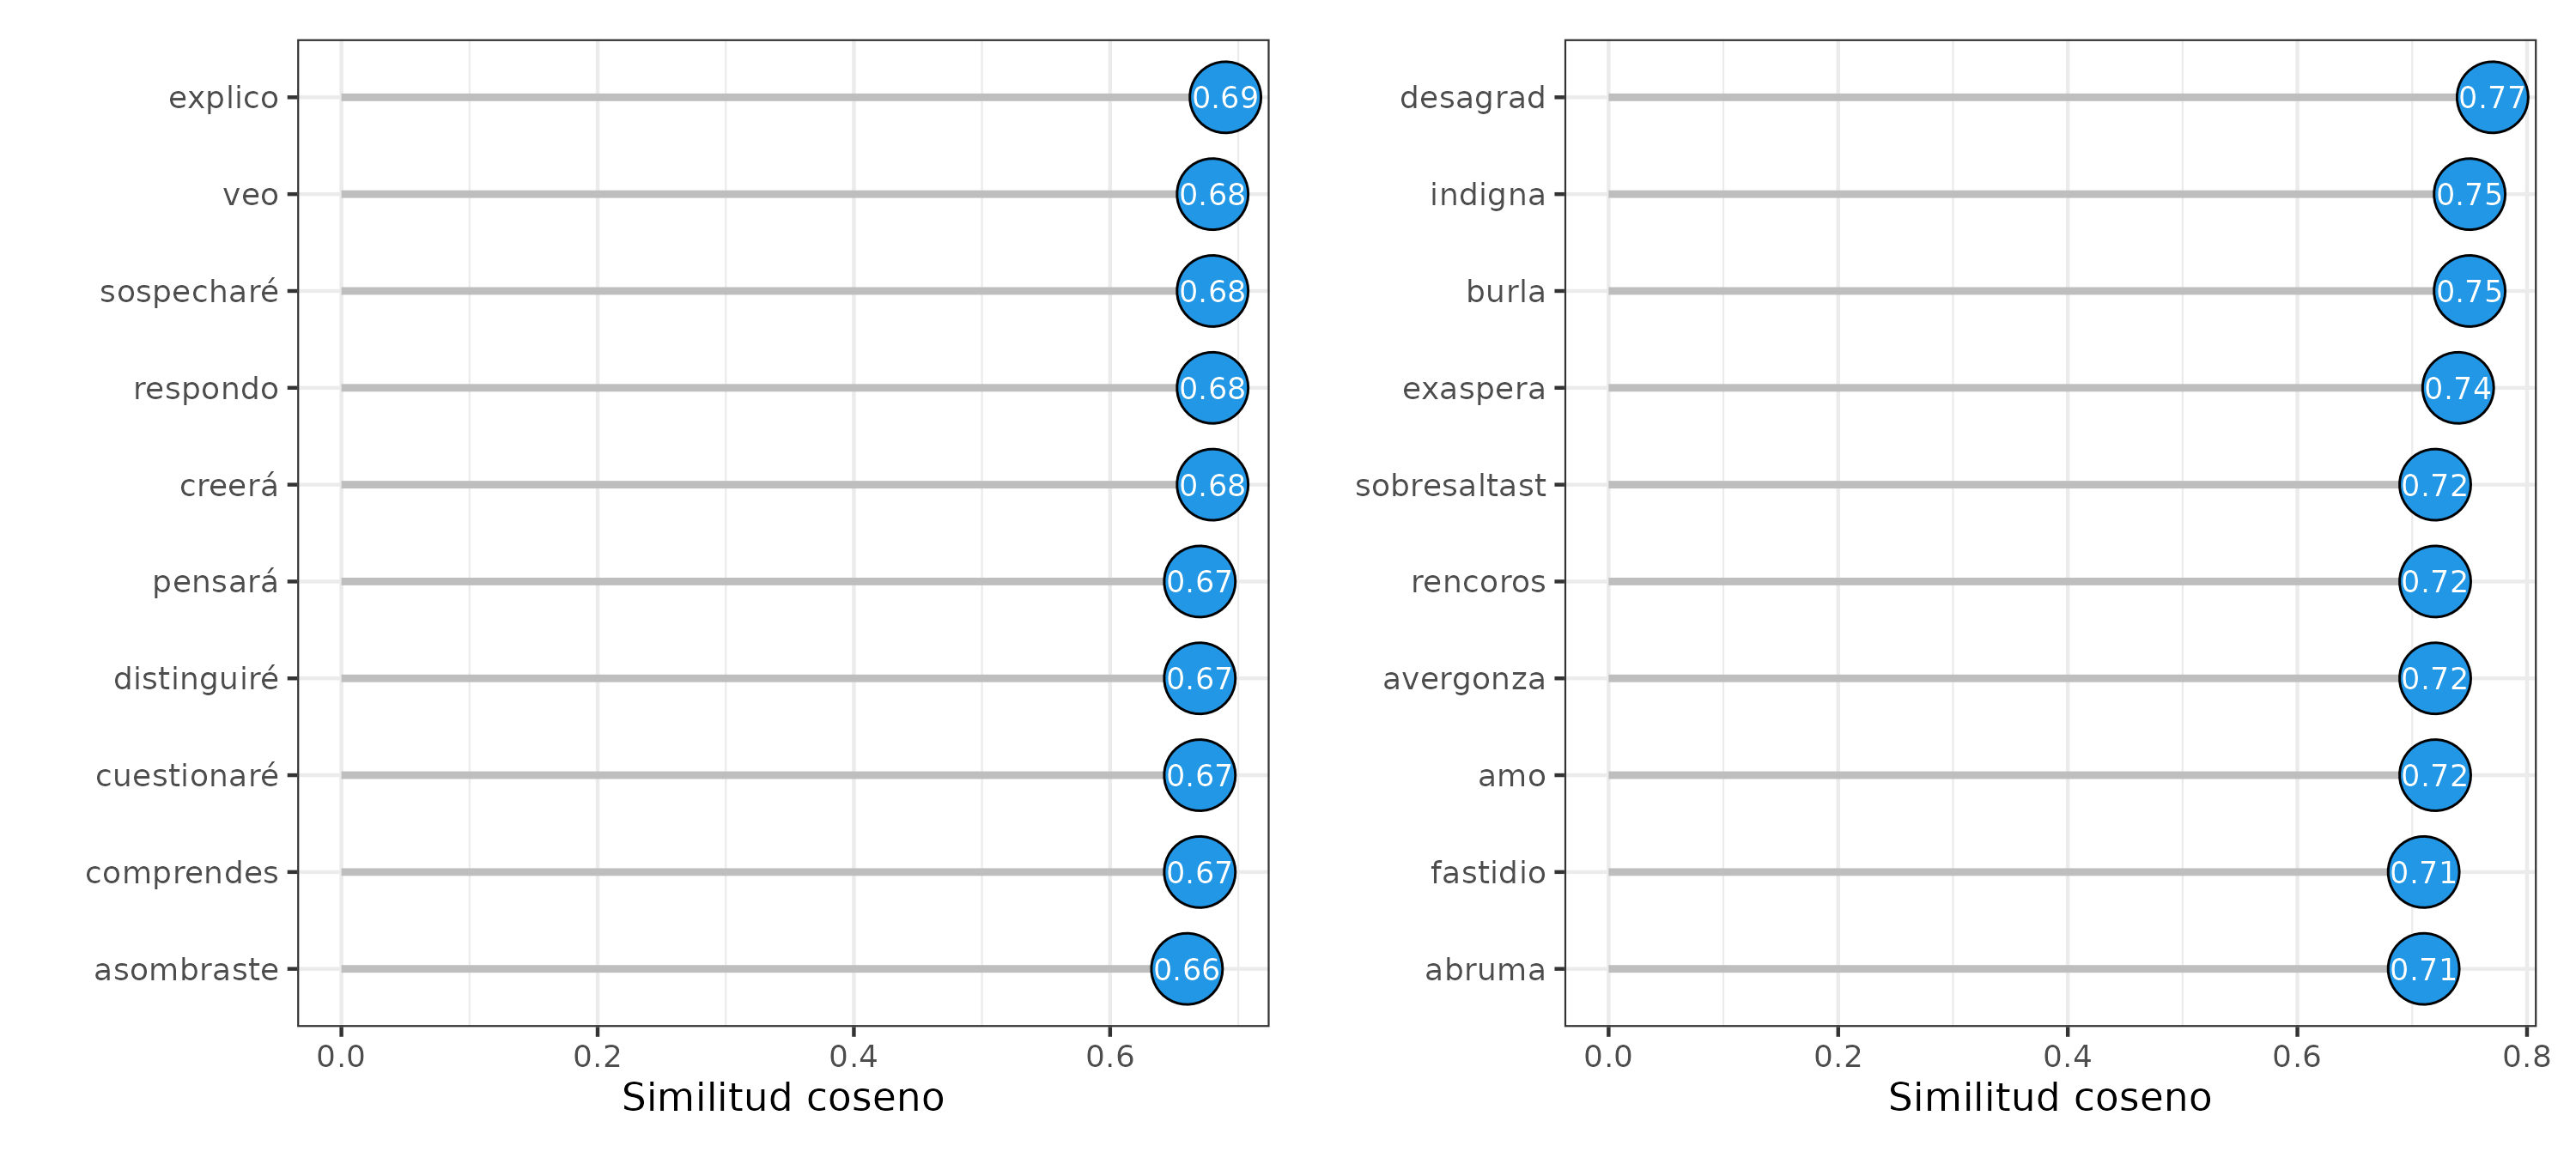
\includegraphics[width = 0.7 \textwidth]{cuadros_tesis/plot_important_words.png}
\end{figure}

Con el objetivo de validar que los vectores efectivamente estén midiendo
afectividad y cognición, es importante observar cuáles son las palabras
del corpus (conjunto de intervenciones políticas) que más se acercan a
cada una de las polaridades. Para ello, se calculó la similitud coseno
entre cada una de las
193.205\footnote{Este número corresponde al total de palabras luego de haber aplicado un procedimiento de \textit{tokenización}, mediante el cual se eliminan \textit{stoptwords} y se seleccionan solo los adjetivos, sustantivos y verbos}
palabras distintas del corpus que no están dentro del diccionario y los
vectores que representan a los polos cognitivo y afectivo. Las figuras
\ref{fig:nube_afectiva} y \ref{fig:nube_cognitiva} muestran (a través de
su tamaño) cuán cerca se encuentra una palabra de cada una de las
polaridades. Se observa que, efectivamente, los vectores construidos
para cada una de las polaridades dan cuenta de afectividad y cognición,
ya que mientras en el panel izquierdo (polaridad afectiva) palabras como
\emph{rencoroso}, \emph{atormentado} y \emph{enfado} muestran
predominancia, en el panel derecho resaltan verbos como \emph{decir},
\emph{demostrar} y \emph{preguntar}.

Cabe mencionar que las palabras del polo afectivo presentan un sesgo
hacia emociones tradicionalmente consideradas como negativas. El motivo
de ello es que LIWC (diccionario utilizado) tiene un sesgo hacia
palabras de este tipo, lo que implica que la construcción del vector de
afectividad esté sesgado hacia ese tipo de emociones, cuestión que debe
tenerse en consideración al momento de analizar los resultados. Con el
objeto de descartar que el polo afectivo esté capturando únicamente
emociones negativas, se llevaron a cabo algunas pruebas con palabras
usualmente consideradas positivas como \emph{amor}, \emph{alegría} o
\emph{risa}. Este ejercicio arrojó como resultado una asociación más
fuerte con el vector emotivo que con el cognitivo, lo que da cuenta de
que si bien existe un sesgo hacia emociones negativas, el instrumento es
capaz de dar cuenta también de emociones
positivas\footnote{Para más detalles sobre estas pruebas, ver el anexo.}.

\begin{figure}[H]
     \caption{Nubes de palabras }
     \centering
     \begin{subfigure}[b]{0.4\textwidth}
         \centering
         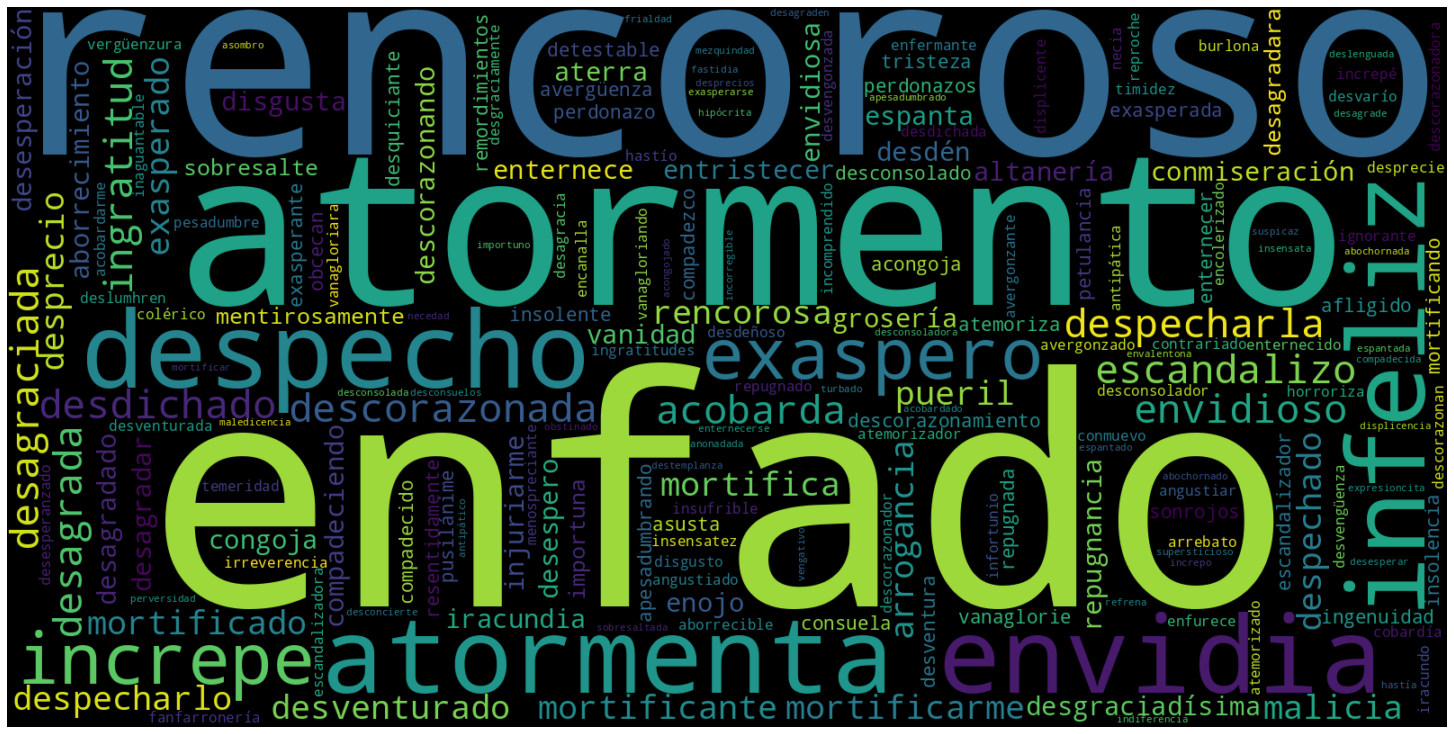
\includegraphics[width=\textwidth]{cuadros_tesis/wordcloud_affective.png}
         \caption{Polo afectivo}
         \label{fig:nube_afectiva}
     \end{subfigure}
     \begin{subfigure}[b]{0.4\textwidth}
         \centering
         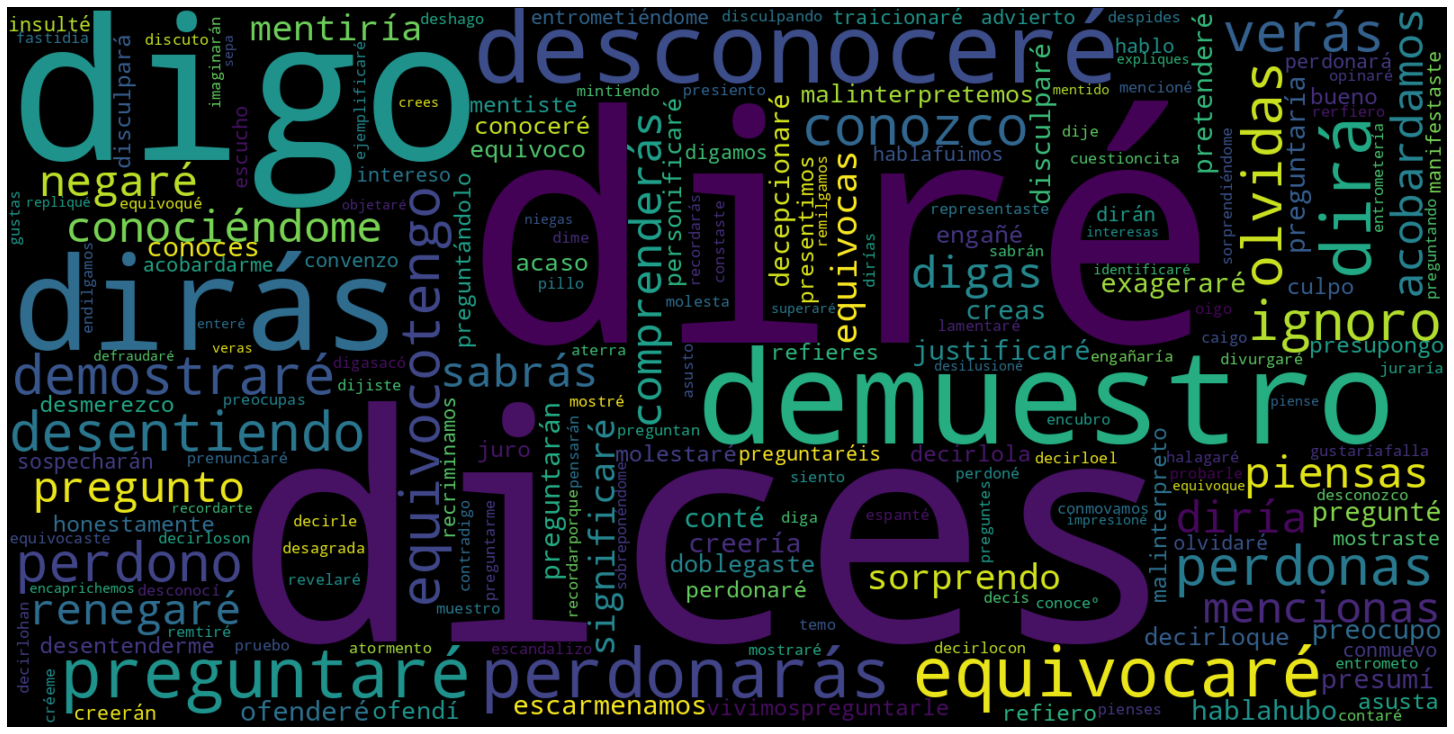
\includegraphics[width=\textwidth]{cuadros_tesis/wordcloud_cognitive.png}
         \caption{Polo cognitivo}
         \label{fig:nube_cognitiva}
     \end{subfigure}
     \label{fig:nubes}
     \caption*{\footnotesize{\textit{Nota:} Cada nube contiene las 200 palabras con mayor similitud coseno respecto a los vectores cognitivo y afectivo. El tamaño de las palabras se pondera de acuerdo al valor de la similitud coseno.}}
\end{figure}

\hypertarget{identificaciuxf3n-de-la-polaridad}{%
\subsection{Identificación de la
polaridad}\label{identificaciuxf3n-de-la-polaridad}}

Para convertir en vectores cada uno de los párrafos que componen las
intervenciones parlamentarias, se implementan los procedimientos
descritos en el apartado \ref{word_emb}. En primer lugar, se busca un
vector para cada una de las palabras que están dentro de un texto.
Luego, para generar un indicador agregado de cada texto, se calcula el
centroide de todas las palabras que lo componen. De esta manera, sin
importar la cantidad de palabras contenidas en un texto, su
representación final será siempre un vector de 100 dimensiones, que
funciona como ``resumen'' del texto original.

Una vez que los más de 2 millones de párrafos son \emph{mapeados} a su
respectivo vector, es posible llevar a cabo todo tipo de operaciones
algebraicas con ellos. Para identificar la polaridad de cada párrafo, se
utiliza la metodología propuesta por (Gennaro y Ash 2021). La idea de
fondo es que un texto puede contener simultáneamente emotividad y
cognición. Ello implica que la medida utilizada debe dar cuenta de dicha
dualidad y generar un valor sintético considerando ambas dimensiones. El
indicador utilizado para medir emocionalidad de un texto es el
siguiente:

\begin{align}
\label{indicador_emotividad}
Y_i = \frac{sim(d_i, A) + b}{sim(d_i, C) + b} 
\end{align}

Donde \textit{A} representa al vector del polo afectivo y \textit{C}, al
vector cognitivo. La expresión
\(sim(v, w) = (v \cdot w)/(||v||\;||w||)\) corresponde a la similitud
coseno entre los vectores \textit{v} y \textit{w}. El término \textit{b}
se introduce para suavizar posibles \emph{outliers} y puede ser
cualquier número positivo pequeño. Respecto a la interpretación, un
incremento en \(Y_i\) corresponde a un movimiento hacia la polaridad
afectiva. Cuando \(Y_i\) toma valor 1 significa que el texto es neutro
en la polaridad afectivo-cognitivo.

Los gráficos de la figura \ref{fig:similitud_polos} muestran las
distribuciones de \(Y_i\), \(sim(d_i, A)\) y \(sim(d_i, C)\). En el
gráfico del panel \ref{fig:sintetico_emocionalidad} se puede observar
que el indicador sintético se mueve aproximadamente entre 0.8 y 1.2, con
una distribución levemente sesgada hacia la derecha, es decir, hacia el
polo afectivo (valores mayores a 1 indican afectividad). Por su parte,
los indicadores parciales de afectividad y cognición se encuentran
centrados en 0.5 y se mueven entre 0 y 1.

\begin{figure}[H]
     \caption{Indicadores de afectividad y cognición}
     \centering
     \begin{subfigure}[b]{0.4\textwidth}
         \centering
         \includegraphics[width=\textwidth]{cuadros_tesis/plot_affective.png}
         \caption{Similitud coseno polo afectivo}
         \label{fig:similitud_afectivo}
     \end{subfigure}
     \begin{subfigure}[b]{0.4\textwidth}
         \centering
         \includegraphics[width=\textwidth]{cuadros_tesis/plot_cognitive.png}
         \caption{Similitud coseno polo cognitivo}
         \label{fig:similitud_cognitiva}
     \end{subfigure}
      \begin{subfigure}[b]{0.6\textwidth}
         \centering
         \includegraphics[width=\textwidth]{cuadros_tesis/plot_scores.png}
         \caption{Indicador sintético de emocionalidad}
         \label{fig:sintetico_emocionalidad}
     \end{subfigure}
     \label{fig:similitud_polos}
     \caption*{\footnotesize{\textit{Nota: blabla} }}
\end{figure}

Con el objeto de entregar evidencia de que el indicador propuesto
funciona, un ejercicio posible es inspeccionar visualmente cómo son los
textos que presentan puntajes elevados en el polo afectivo y cognitivo,
respectivamente. En los cuadros \ref{tab:tabla_frases_cognitivas} y
\ref{tab:tabla_frases_afectivas} se muestran las 15 frases con mayor
puntaje en el polo cognitivo y afectivo. Una lectura rápida muestra que,
efectivamente, el indicador está dando cuenta de la polaridad que se
pretende medir. En el caso del cuadro \ref{tab:tabla_frases_cognitivas}
se observan verbos como analizar, fijar, buscar, modificar, decidir, que
de alguna manera se asocian a actividades con un fuerte componente
cognitivo. Por su parte, la tabla \ref{tab:tabla_frases_cognitivas}
contiene palabras como sensación, inseguridad, brutal, desorden,
anarquía, etc, es decir, palabras que apuntan hacia una dimensión
afectiva.

\begin{table}[H]

\caption{\label{tab:tabla_frases_cognitivas}15 frases más cognitivas}
\centering
\fontsize{10}{12}\selectfont
\begin{tabular}[t]{>{\raggedright\arraybackslash}p{25em}}
\toprule
text\\
\midrule
\em{\textbf{- después fijaremos la fecha exacta.}}\\
\em{\textbf{- más adelante analizaré los otros artículos del proyecto.}}\\
\em{\textbf{- los numerales de que consta son los siguientes.}}\\
\em{\textbf{- eso es lo que tenemos y lo que buscamos modificar.}}\\
\em{\textbf{- aquí efectuamos una modificación que señalaré más adelante.}}\\
\addlinespace
\em{\textbf{- aquí dijimos revisemos esto veamos qué ocurre.}}\\
\em{\textbf{- porque cambiamos la ubicación de ese artículo.}}\\
\em{\textbf{- ¡si no los tenemos ahora ni los tendremos mañana si no llegamos a acuerdo.}}\\
\em{\textbf{- entonces votamos y establecemos un plazo para las.}}\\
\em{\textbf{- además tenemos proyectos aprobados.}}\\
\addlinespace
\em{\textbf{- que los pocos instrumentos que tenemos los utilizaremos para llegar a un acuerdo con el gobierno eso haremos.}}\\
\em{\textbf{- corresponden a las indicaciones números 233 y 234.}}\\
\em{\textbf{- eso lo discutiremos cuando llegue el texto respectivo.}}\\
\em{\textbf{- tenemos que analizar cómo lo hacemos para adelante.}}\\
\em{\textbf{- vamos a decidir si sacamos o no de la tabla el proyecto.}}\\
\bottomrule
\end{tabular}
\end{table}

\begin{table}[H]

\caption{\label{tab:tabla_frases_afectivas}15 frases más afectivas}
\centering
\fontsize{10}{12}\selectfont
\begin{tabular}[t]{>{\raggedright\arraybackslash}p{25em}}
\toprule
text\\
\midrule
\em{\textbf{- desocupación de los jóvenes un 30 por ciento de la población juvenil.}}\\
\em{\textbf{- la sensación de inseguridad en la población.}}\\
\em{\textbf{- sea una indolencia brutal total.}}\\
\em{\textbf{- sembrando un clima de inquietud de inseguridad de violencia.}}\\
\em{\textbf{- entonces más fragmentación más inestabilidad más desgobierno.}}\\
\addlinespace
\em{\textbf{- para alentarlos al desorden y a la anarquía.}}\\
\em{\textbf{- a con esfuerzo físico excesivo.}}\\
\em{\textbf{- en consecuencia con el mismo ánimo solidario reflejo mi preocupación por aquello.}}\\
\em{\textbf{- acá hay lluvias en demasía y sequías excesivas hay falta de agua en el verano y exceso en el invierno.}}\\
\em{\textbf{- f la campaña del terror desatada por los latifundistas.}}\\
\addlinespace
\em{\textbf{- sin el ánimo de disminuir la importancia de la iniciativa.}}\\
\em{\textbf{- además ésa es una inquietud de numerosos sectores de nuestra ciudadanía.}}\\
\em{\textbf{- esta situación ha contribuido a la exacerbación y recrudecimiento de otros males socialmente nefastos creando un clima de inseguridad desconfianza y desesperanza.}}\\
\em{\textbf{- ¡eso y no el boicot es lo que está provocando la escasez de alimentos.}}\\
\em{\textbf{- cierta hilaridad es manifestación de nerviosismo.}}\\
\bottomrule
\end{tabular}
\end{table}

Para aportar más información respecto al funcionamiento del indicador,
las siguientes figuras muestran un resumen de los 5.000 textos con mayor
puntaje cognitivo y 5.000 con mayor puntaje afectivo. El ejercicio
consiste en calcular la frecuencia de las palabra de cada uno de los
conjuntos de datos (luego de haber removido las \emph{stopwords}) y
graficar dicha información mediante nubes de palabras. Así, palabras de
mayor tamaño reflejan una alta frecuencia y viceversa. Se puede observar
que mientras en el polo cognitivo resaltan palabras como proyecto,
artículo, o indicación, en el polo afectivo se observan palabras como
manifestaciones, aplausos y violencia.

\begin{figure}[H]
     \caption{5.000 frases más cognitivas y afectivas}
     \centering
     \begin{subfigure}[b]{0.4\textwidth}
         \centering
         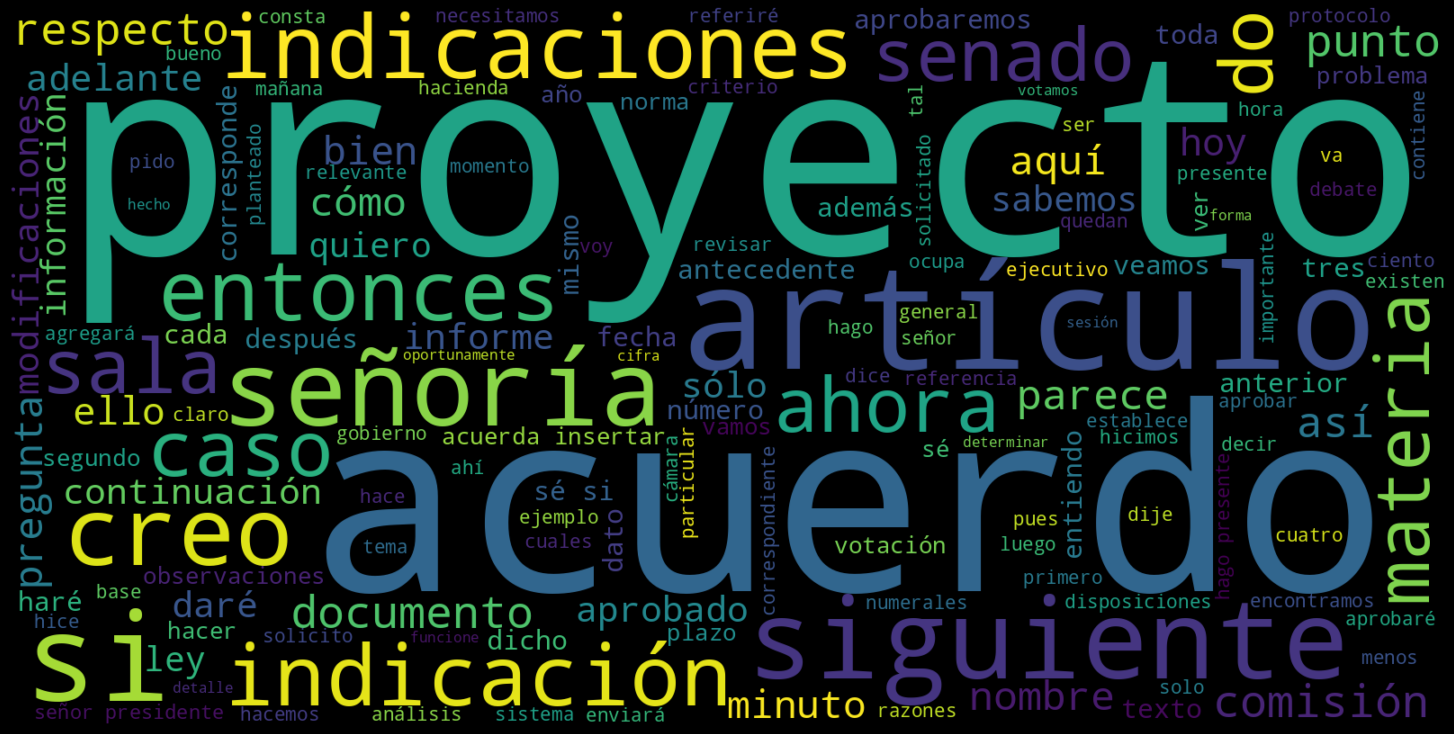
\includegraphics[width=\textwidth]{cuadros_tesis/wordcloud_most_cognitive_phrases.png}
         \caption{Palabras polo cognitivo}
         \label{fig:cognitive_5000}
     \end{subfigure}
     \begin{subfigure}[b]{0.4\textwidth}
         \centering
         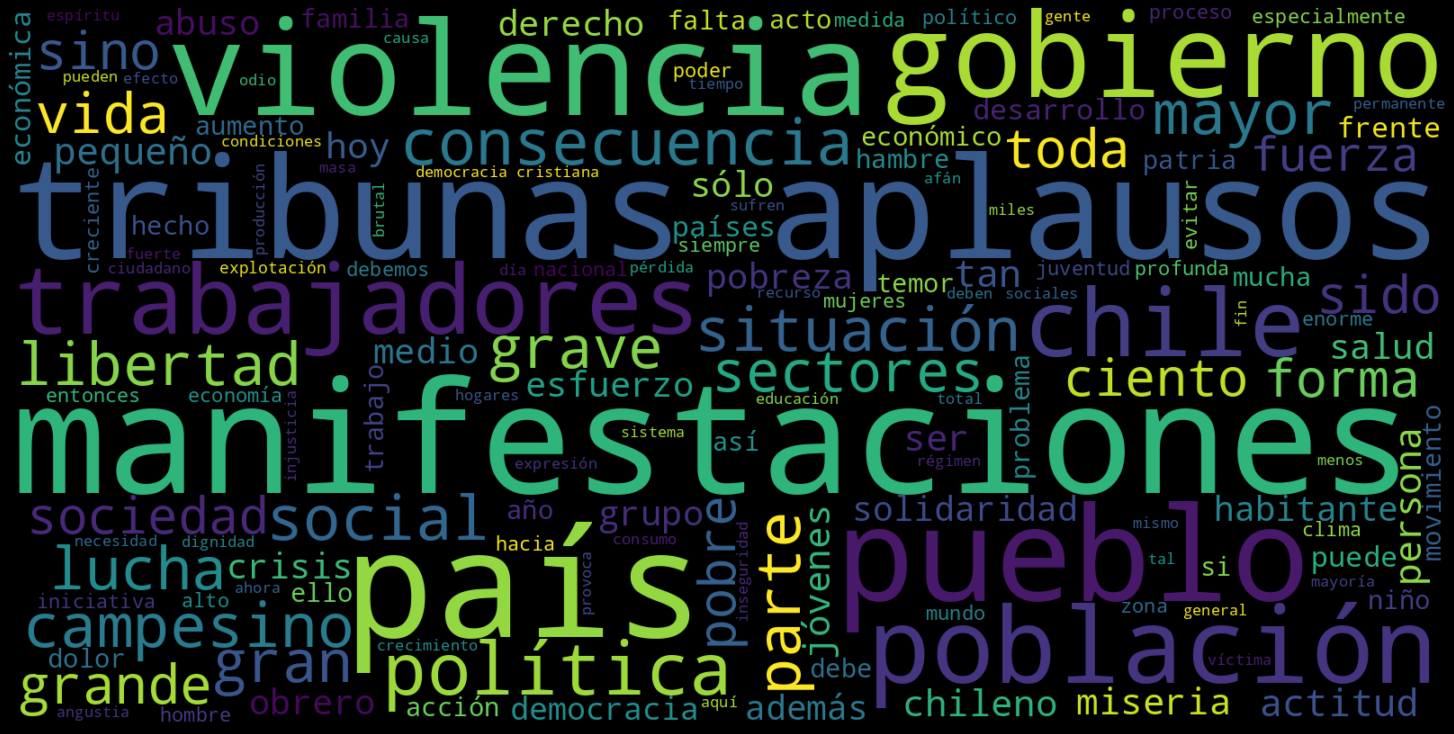
\includegraphics[width=\textwidth]{cuadros_tesis/wordcloud_most_afective_phrases.png}
         \caption{Palabras polo afectivo}
         \label{fig:affective_5000}
     \end{subfigure}
     \label{fig:1000_phrases}
     \caption*{\footnotesize{\textit{Nota: Fueron removidas las \textit{stoptwords} para mejorar la visualización. Cada nube contiene un máximo de 150 palabras} }}
\end{figure}

Un último ejercicio para evaluar el indicador consiste en comprobar si
la agrupación de palabras mostrada en las nubes de palabras (figura
\ref{fig:1000_phrases}) tiene un correlato en términos espaciales. Si el
indicador utilizado realmente refleja dos polaridades, debería ser capaz
de discriminar entre diferentes tipos de contenido textual y generar
agrupaciones. En ese sentido, es posible seleccionar la representación
vectorial construida mediante \emph{word embeddings} (100 dimensiones)
de los los textos con mayor puntaje cognitivo y afectivo (1.000 por
polaridad), y proyectar ese espacio de 100 dimensiones en uno de 2,
mediante PCA. La figura \ref{scatter_embedding} da cuenta de que pese a
que se ha reducido de 100 a 2 dimensiones, la información conservada es
capaz de generar una agrupación de textos coherente, ya que
efectivamente los textos con contenido afectivo y cognitivo ocupan
espacios que no se superponen.

\begin{figure}[H]
\centering
\large
\caption{Proyección en dos dimensiones de los mil primeros textos cognitivos y afectivos}
\label{scatter_embedding}
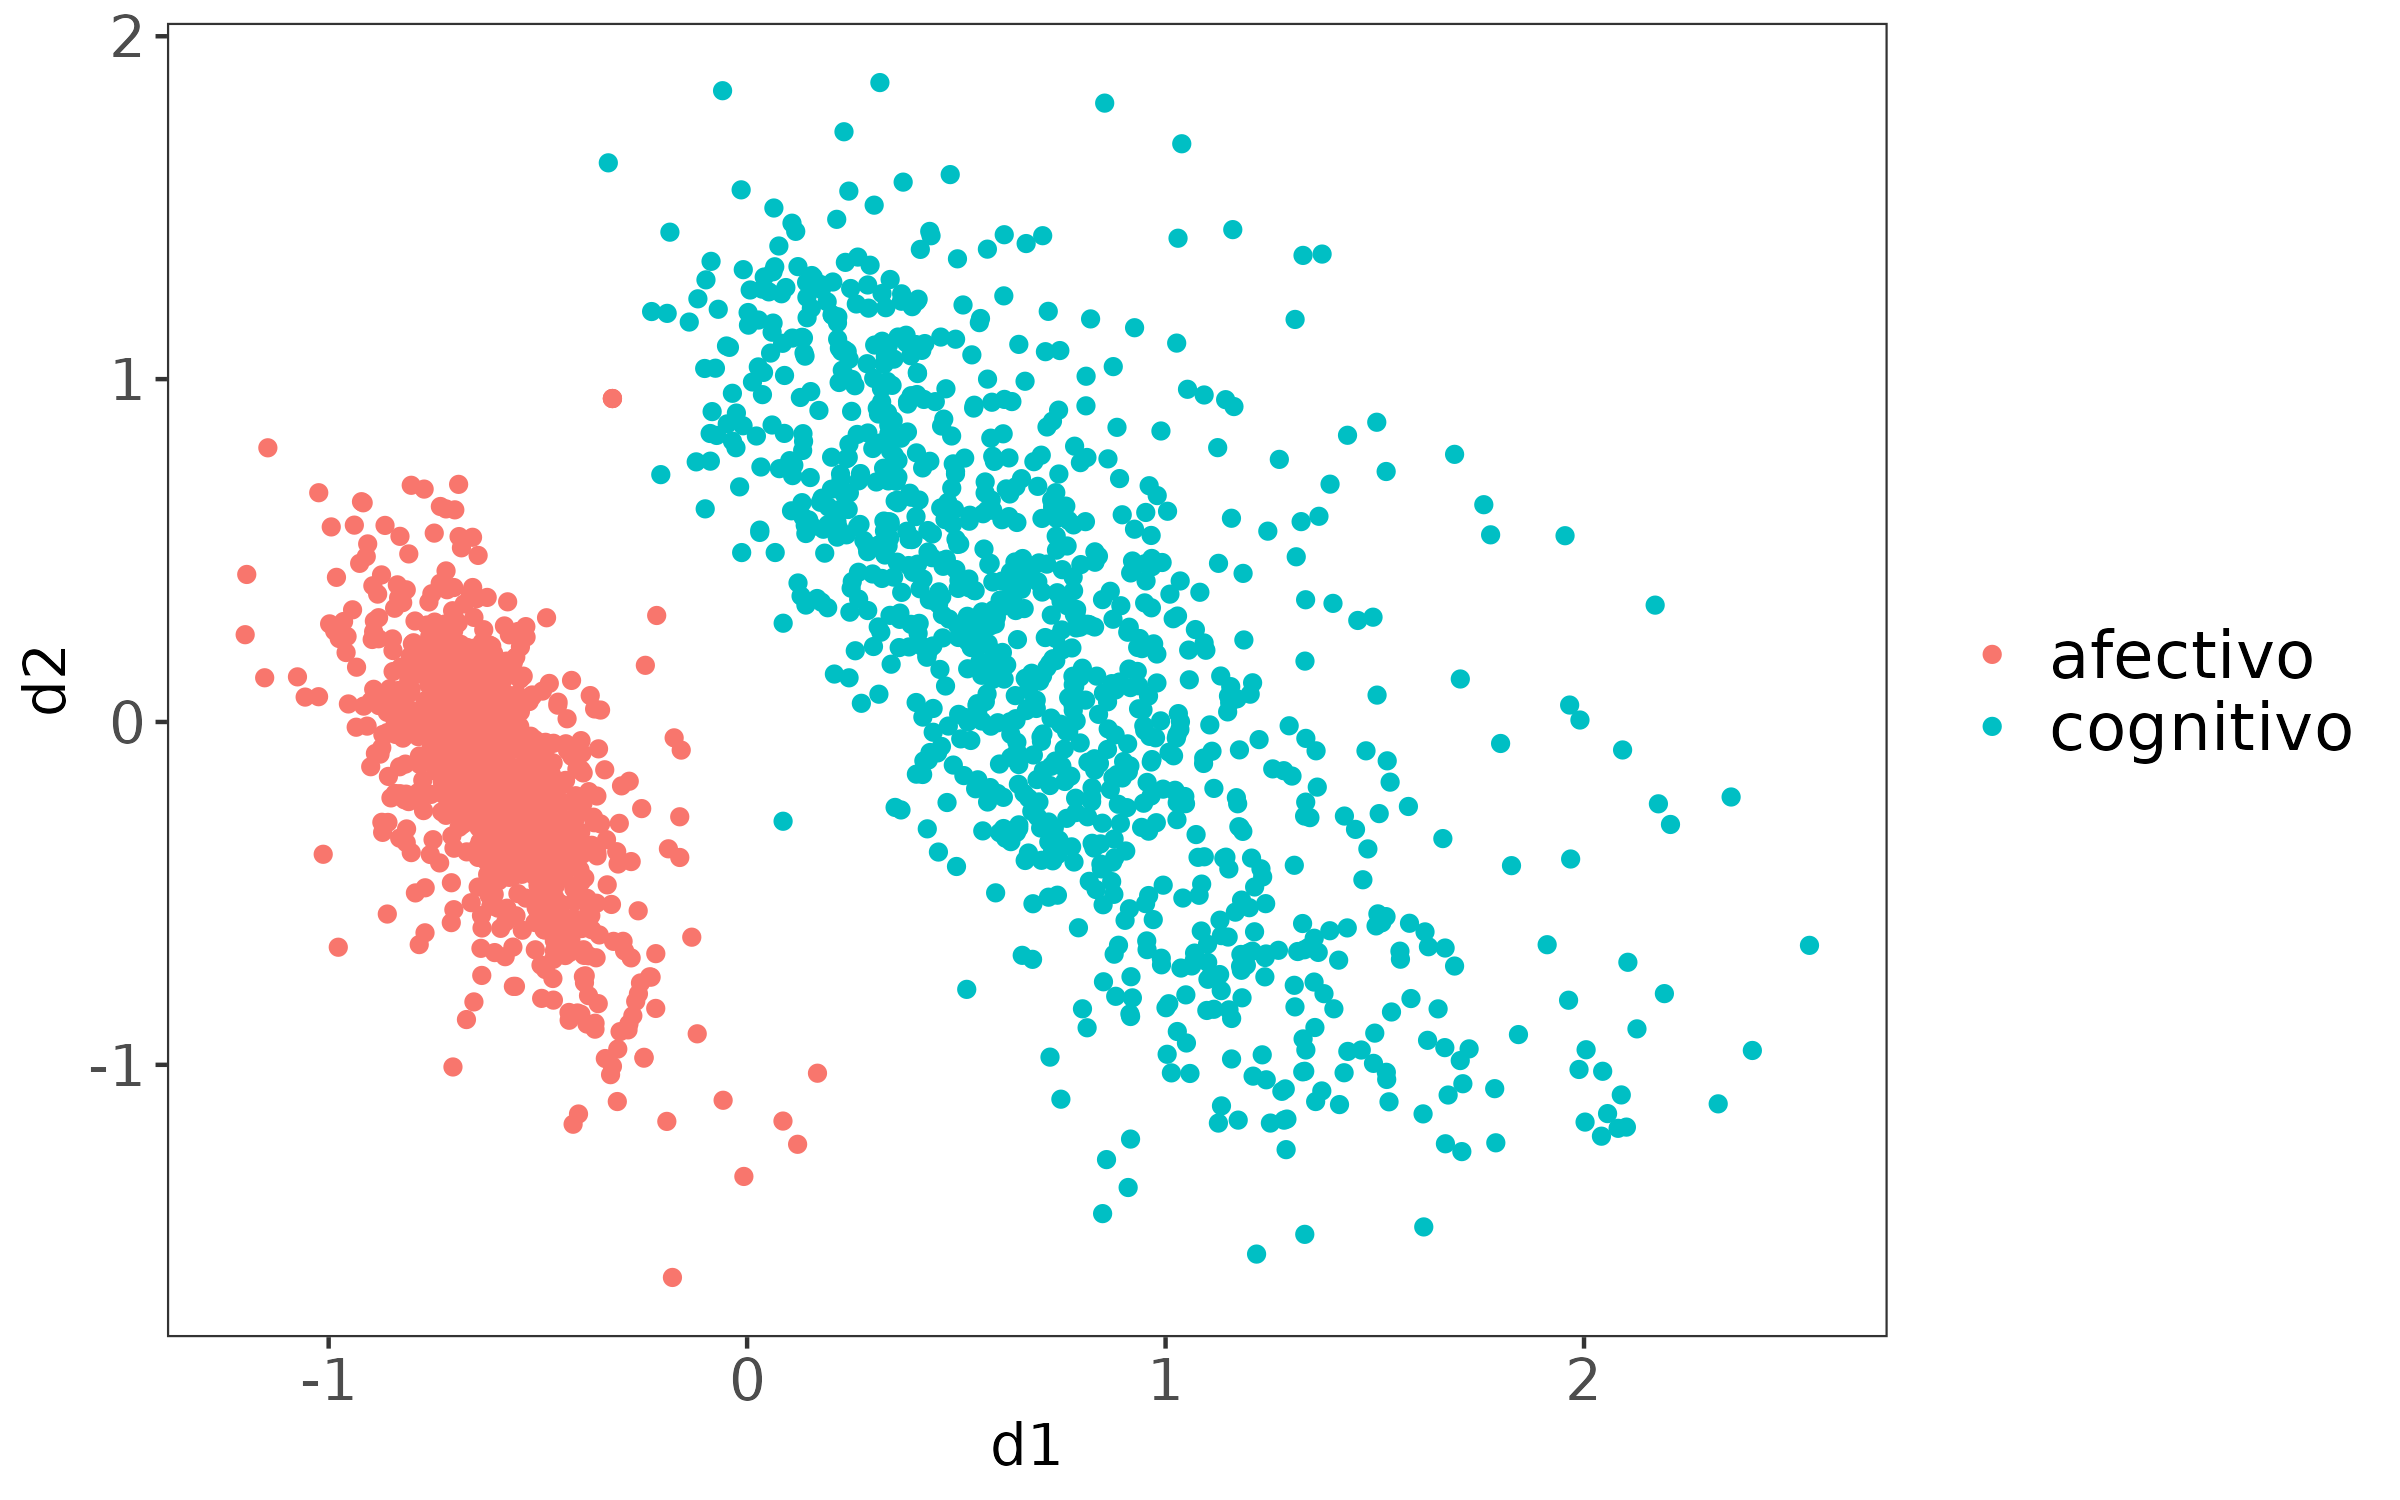
\includegraphics[width = 0.5 \textwidth]{cuadros_tesis/polarity_scatter_plot.png}
\normalsize
\end{figure}

\hypertarget{identificaciuxf3n-de-tuxf3picos}{%
\subsection{Identificación de
tópicos}\label{identificaciuxf3n-de-tuxf3picos}}

La identificación de tópicos se realizó mediante un modelo basado en
ELECTRA
\footnote{El modelo original fue bautizado como ELECTRA y SELECTRA corresponde a su versión en español.},
al cual se le aplicó un procedimiento de \emph{fine-tuning} para la
tarea específica de detectar tópicos. Esta arquitectura (Clark et~al.
2020) está compuesta por dos redes: red generadora y red discriminadora.
La primera es entrenada para predecir una palabra a partir de su
contexto, mientras que la segunda (red discriminadora) recibe un
entrenamiento para discriminar si una palabra corresponde a un dato
sintético (una predicción de la red generativa) o a un dato original.
Tal como señalan Clark et~al. (2020), este modelo presenta
reminiscencias de las redes generativas adversarias (GAN), sin embargo,
existen algunas diferencias que la distancian de dicho diseño.

El modelo recibe como entrada un texto y una serie de tópicos
considerados relevantes. La respuesta consiste en un vector que contiene
la probabilidad que la red le asigna a cada tópico. Para cada texto se
seleccionó el tópico con probabilidad más alta, el cual se usó como
etiqueta. Los tópicos considerados fueron: 1) salud, 2) educación, 3)
deporte, 4) medioambiente, 5) impuestos, 6) cultura, 7) pensiones, 8)
sindicalismo, 9) transporte, 10) familia y 11) aborto.

\hypertarget{polarizaciuxf3n-poluxedtica}{%
\subsection{\texorpdfstring{Polarización política
\label{apartado_nominate}}{Polarización política }}\label{polarizaciuxf3n-poluxedtica}}

Para incluir una medida de polarización política se utilizó un modelo
proveniente de la ciencia política llamado W-NOMINATE, cuya formulación
inicial fue realizada por Poole y Rosenthal
(1983)\footnote{El modelo inicial de Poole y Rosenthal fue bautizado como NOMINATE. Con el tiempo comenzaron a surgir variaciones de la idea original, lo que dio lugar a los modelos D-NOMINATE, W-NOMINATE t DW-NOMINATE. En la actualidad, W-NOMINATE es el más utilizado y, por ende, con implementaciones en lenguajes de programación}
que permite posicionar a cada político en un continuo ideológico a
partir de sus votaciones en el congreso.

La idea central del modelo es que los legisladores tienen un punto
ideológico ideal, de modo que mediante sus decisiones de voto intentarán
minimizar la distancia respecto a dicho punto ideal. Poole y Rosenthal
proponen que la función de utilidad de los políticos depende de un
componente determinístico y de un componente de shocks aleatorios. Se
asume que las personas intentarán maximizar su utilidad, mediante
votaciones que minimicen la distancia respecto a su punto ideal, sujeto
a un componente aleatorio.

Considerando estas ideas, la utilidad \emph{U} del legislador \emph{i}
en la votación \emph{j}, por haber votado afirmativamente (representado
por el subíndice \(y\)) es:

\begin{align}
\label{formula_poole}
U_{ijy} = u_{ijy} + \epsilon_{ijy} \\
u_{ijy} = \beta exp[\frac{\sum_{k=1}^{s}w_{k}^2d_{ijyk}^2 }{2}] 
\end{align}

\(u_{ijy}\) representa la parte determínistica de la utilidad del
legislador, mientras que \(\epsilon_{ijy}\) representa el componente
estocástico. El término \(d_{ijyk}^2\) es la distancia euclidiana entre
el punto ideal \(x_i\) del político en la dimensión \(k\) y la posición
\(z_{jyk}\) resultante de haber votado afirmativamente el proyecto de
ley:

\begin{align}
\label{formula_distancia}
d_{ijyk}^2 = \sum_{k=1}^{s}(x_{ik} - z_{jyk})^2)
\end{align}

Tanto el peso \(w\) como \(\beta\) deben ser estimados, partiendo de
valores de 0.5 y 15, respectivamente. \(w\) representa la poderación de
cada dimensión política, mientras que el término \(\beta\) corresponde a
la importancia que tiene la parte determinística de la utilidad. Así,
valores altos de \(\beta\) implican una pérdida de relevancia del
componente aleatorio.

Si bien el modelo puede utilizarse para obtener, \(s\) cantidad de
dimensiones, por lo general se utilizan las dos primeras, ya que se ha
demostrado empíricamente que no se requiere más que ello para generar
agrupaciones coherentes. De hecho, en muchos casos es suficiente la
primera dimensión para resumir el comportamiento político de las
coaliciones. En ese sentido, el modelo puede ser entendido como
estrategia de reducción de dimensionalidad, ya que típicamente se parte
con cientos o miles de votaciones, las cuales son reducidas a una o 2
dimensiones.

A continuación, se muestran los puntajes promedio obtenidos para algunos
de los partidos más relevantes a nivel nacional a lo largo de todo el
periodo disponible. Se observa que la primera dimensión del modelo
genera una agrupación satisfactoria respecto a la tradición política de
los últimos 20. El posicionamiento de los partidos de derecha (RN, UDI y
EVOPOLI) y de izquierda (PS, PPD, RD, PCS, PC) refleja relativamente
bien la configuración ideológica de la Cámara de Diputados. Es
interesante notar que el modelo es capaz de dar cuenta de movimientos en
el comportamiento de los partidos, como por ejemplo, el caso de la
Democracia Cristiana (DC), cuyo posicionamiento pasa desde un
alineamiento con los partidos de izquierda y centro izquierda, hacia un
viraje hacia la derecha en los últimos años.

\begin{figure}[H]
\centering
\large
\caption{W-NOMINATE: Puntaje promedio por partido de la primera dimensión}
\label{w_nominate_plot}
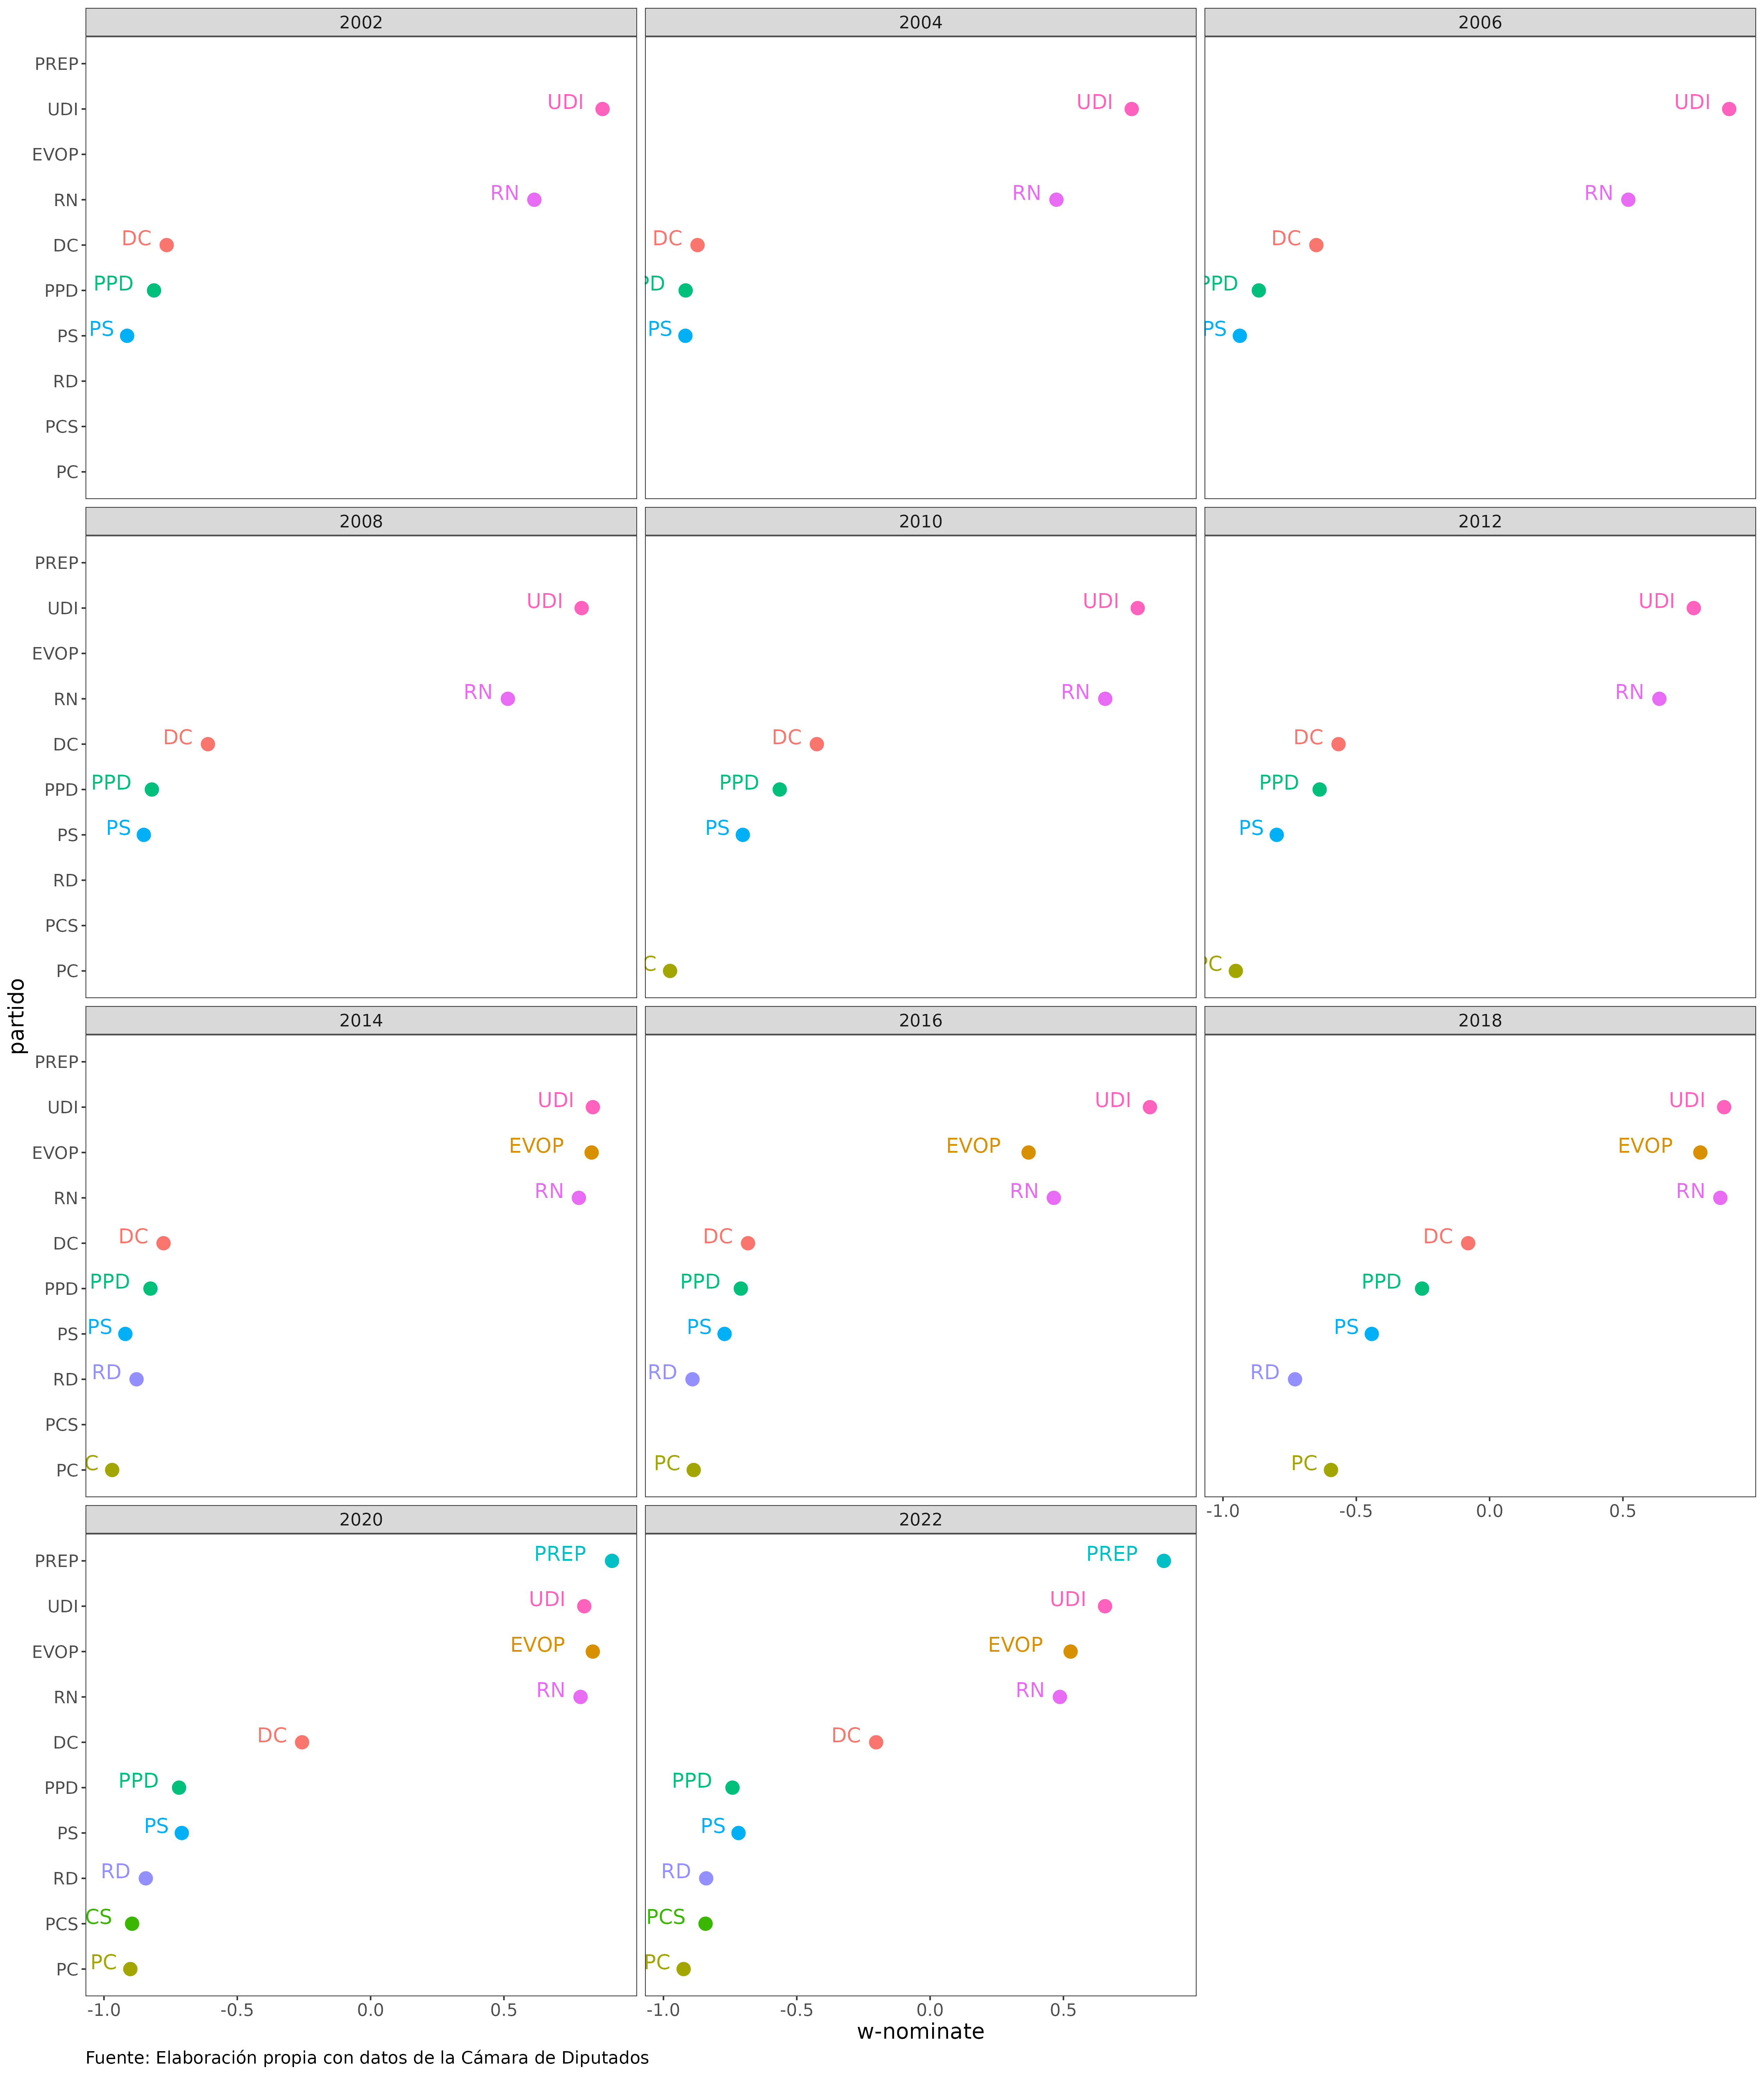
\includegraphics[width = 0.9 \textwidth]{cuadros_tesis/nominate_partido_anio.png}
\normalsize
\end{figure}

Para efectos de este trabajo, se utilizan medidas agregadas de
posicionamiento político, clasificando a cada parlamentario en las
categorías izquierda y derecha. La figura \ref{w_nominate_hist} muestra
los puntajes del modelo para el año 2021, considerando los mismos
partidos del gráfico anterior, pero ahora a nivel de cada parlamentario.
Se observa que los polos de izquierda y derecha se encuentran bien
definidos y que existe una pequeña parte en la que se produce
convergencia entre ambas polos, lo cual se explica principalmente por el
posicionamiento de los parlamentarios del Partido Demócrata Cristiano.
Ello se observa con bastante claridad en la figura
\ref{w_nominate_scatter}, donde los puntos rojos corresponde a la
posición de los parlamentarios de dicha colectividad en un espacio de
dos dimensiones.

\begin{figure}[H]
\centering
\large
\caption{W-NOMINATE: Puntaje promedio por parlamentario de la primera dimensión}
\label{w_nominate_hist}
\includegraphics[width = 0.5 \textwidth]{cuadros_tesis/nominate_histograma.png}
\normalsize
\end{figure}

\begin{figure}[H]
\centering
\large
\caption{W-NOMINATE: Puntaje promedio por parlamentario de las dos primeras dimensiones}
\label{w_nominate_scatter}
\includegraphics[width = 0.5 \textwidth]{cuadros_tesis/nominate_scatter.png}
\normalsize
\end{figure}

\hypertarget{resultados}{%
\section{Resultados}\label{resultados}}

\hypertarget{estaduxedstica-descriptiva-polos-y-tuxf3picos}{%
\subsection{Estadística descriptiva polos y
tópicos}\label{estaduxedstica-descriptiva-polos-y-tuxf3picos}}

\hypertarget{regresiuxf3n}{%
\subsection{Regresión}\label{regresiuxf3n}}

\hypertarget{conclusiones}{%
\section{Conclusiones}\label{conclusiones}}

Mis grandes conclusiones

\newpage

\hypertarget{referencias}{%
\section*{Referencias}\label{referencias}}
\addcontentsline{toc}{section}{Referencias}

\hypertarget{refs}{}
\begin{CSLReferences}{1}{0}
\leavevmode\vadjust pre{\hypertarget{ref-fasttext}{}}%
Bojanowski, Piotr, Edouard Grave, Armand Joulin, y Tomás Mikolov. 2016.
{«Enriching Word Vectors with Subword Information»}. \emph{CoRR}
abs/1607.04606. \url{http://arxiv.org/abs/1607.04606}.

\leavevmode\vadjust pre{\hypertarget{ref-aggarwal}{}}%
Charu C., Aggarwal. 2018. \emph{Neural Networks and Deep Learning. A
Textbook}. Springer Cham.
https://doi.org/\url{https://doi.org/10.1007/978-3-319-73004-2}.

\leavevmode\vadjust pre{\hypertarget{ref-electra}{}}%
Clark, Kevin, Minh-Thang Luong, Quoc V. Le, y Christopher D. Manning.
2020. {«{ELECTRA:} Pre-training Text Encoders as Discriminators Rather
Than Generators»}. En \emph{8th International Conference on Learning
Representations, {ICLR} 2020, Addis Ababa, Ethiopia, April 26-30, 2020}.
OpenReview.net. \url{https://openreview.net/forum?id=r1xMH1BtvB}.

\leavevmode\vadjust pre{\hypertarget{ref-paper_central}{}}%
Gennaro, Gloria, y Elliott Ash. 2021. {«{Emotion and Reason in Political
Language}»}. \emph{The Economic Journal} 132 (643): 1037-59.
\url{https://doi.org/10.1093/ej/ueab104}.

\leavevmode\vadjust pre{\hypertarget{ref-bing}{}}%
Hu, Minqing, y Bing Liu. 2004. {«Mining and summarizing customer
reviews»}.
\url{https://www.cs.uic.edu/~liub/publications/kdd04-revSummary.pdf}.

\leavevmode\vadjust pre{\hypertarget{ref-vader}{}}%
Hutto, C. J., y E. E Gilbert. 2014. {«VADER: A Parsimonious Rule-based
Model for Sentiment Analysis of Social Media Text. Eighth International
Conference on Weblogs and Social Media (ICWSM-14)»}.
\url{https://ojs.aaai.org/index.php/ICWSM/article/view/14550/14399}.

\leavevmode\vadjust pre{\hypertarget{ref-afinn}{}}%
Nielsen, F. Å. 2011. {«AFINN»}. Richard Petersens Plads, Building 321,
{DK-}2800 Kgs. Lyngby: Informatics; Mathematical Modelling, Technical
University of Denmark.
\url{http://www2.compute.dtu.dk/pubdb/pubs/6010-full.html}.

\leavevmode\vadjust pre{\hypertarget{ref-linguistic_dictionary}{}}%
Pennebaker, J. W., R. L. Boyd, K. Jordan, y K. Blackburn. 2015.
\emph{The development and psychometric properties of LIWC2015}. Austin,
TX: University of Texas at Austin.
\url{https://www.liwc.app/static/documents/LIWC2015\%20Manual\%20-\%20Development\%20and\%20Psychometrics.pdf}.

\leavevmode\vadjust pre{\hypertarget{ref-word_embeddings}{}}%
Perez, Jorge, y José Cañete. 2019. {«Spanish Word Embeddings»}.
\url{https://github.com/dccuchile/spanish-word-embeddings}.

\leavevmode\vadjust pre{\hypertarget{ref-nominate}{}}%
Poole, Keith, y Howard Rosenthal. 1983. {«A Spatial Model for
Legislative Roll Call Vote Analysis»}. \emph{American Journal of
Political Science} 29 (agosto). \url{https://doi.org/10.2307/2111172}.

\leavevmode\vadjust pre{\hypertarget{ref-intro_deep_learning}{}}%
Skansi, Sandro. 2018. \emph{Introduction to Deep Learning. From Logical
Calculus to Artificial Intelligence}. Springer Cham.
https://doi.org/\url{https://doi.org/10.1007/978-3-319-73004-2}.

\end{CSLReferences}

\end{document}
